% !TeX spellcheck = cs_CZ
% file: kap_zakld_zakn_elmag.tex
%{\tikzset{external/prefix={tikz/TEO/}}
% \tikzset{external/figure name/.add={ch02_}{}}
%====================Kapitola: Základní zákony elektromagnetismu====================================
\setchaptertoc
\chapter{Základní zákony elektromagnetismu}\label{teo:IchapII}
  V této teoreticky změřené kapitole budou shrnuty základní fyzikální zákony, kterými se řídí
  elektromagnetické jevy a jejichž znalost bude nezbytná při studiu následujících praktičtěji
  zaměřených kapitol. Mezi nejdůležitější patří zákon elektromagnetické indukce. Velký praktický
  význam má jeho zobecnění i pro případy nejsložitější, jakými jsou \emph{nelineární} a navíc
  \emph{parametrické} magnetické obvody. Důležitým pojmem je \emph{spřažený} magnetický tok cívky.
  Pro hlubší pochopení všech zákonitostí bude vhodné upozornit na \emph{topologické vlastnosti}
  elektromagnetického pole. Ukazuje se totiž, že topologický přístup je velice užitečným a silným
  nástrojem, který významně usnadňuje pochopení
  \href{http://en.wikipedia.org/wiki/Maxwell_theory}{Maxwellových rovnic} se všemi jejich důsledky
  \cite[s.~6]{Patocka4}. Topologii elektromagnetického pole je proto věnována celá kapitola
  \ref{teo:IchapIII}
  
  \section{Zákon elektromagnetické indukce}\label{teo:IchapIIsecI}
    Základní veličinou pro popis magnetických polí a jejich účinků je \emph{vektor magnetické
    indukce} \(\vec{B}\). Dle soustavy SI je jednotkou magnetické indukce \emph{tesla} \([T]\) a
    projevuje se silovými účinky na vodiče protékané proudy a indukováním napětí při jeho změně.

    Je proto dobře měřitelný. První rovnice (Ampérův zákon) ze souboru Maxwellových rovnic určuje
    rovnost oběhového integrálu magnetické indukce po uzavřené křivce proudům protékaných vodiči,
    jež jsou touto křivkou uzavřeny.
    \begin{equation}\label{es:eq_amp_law}
      \oint_l \vec{B} \cdot \vec{dl} = \sum I
    \end{equation}
    
    \luagraphic[0.6]{teo_fig034.pdf}{Elektrický proud ve vodiči způsobuje vznik magnetické pole v 
      jeho okolí.}{teo:fig034}

    Obrázek \ref{teo:fig034} ilustruje fakt, že elektrické proudy jsou vždy obklopeny 
    magnetickými poli. Tato pole se dají zesílit cívkou s magnetickým jádrem. Na tomto jevu je 
    založen jeden z elementárních principů elektrotechniky.    
       
    \begin{mdframed}[style=mdnote]
      Jaký je vztah jednotky magnetické indukce k ostatním základním jednotkám soustavy \textbf{SI}? 
      \begin{align*}
      1T &= 1\frac{V\cdot s}{m^2} = 1\frac{N}{A\cdot m} = 1\frac{Wb}{m^2}          \\
         &= 1\frac{kg}{C\cdot s} = 1\frac{kg}{A\cdot s^2} = 1\frac{N\cdot s}{C \cdot m}
      \end{align*}
    \end{mdframed}
    
    Při odvozování matematického modelu transformátoru se obvykle vychází ze zákona 
    \textbf{elektromagnetické indukce}, který říká, že \emph{časová změna magnetického pole vytvoří 
    vírové pole elektrické}:
    \begin{equation}\label{es:eq_ind_z}
      \oint_l \vec{E} \cdot \dd{\vec{l}} = - \der{\Psi}{t}
    \end{equation}
     
    Základní laboratorní experimenty, vedoucí k odhalení existence tohoto zákona, uskutečnil 
    \emph{Faraday}\footnote{Michael Faraday (1791 - 1867), samouk, zakladatel klasické 
    elektrodynamiky, vynikající experimentátor: Zavedl pojem fyzikálního prostorového pole pomocí 
    siločár, tzv. ''trubic''} r. 1831. Matematickou formulaci \emph{indukčního zákona} v podobě 
    rovnice
    \begin{equation}\label{ES:eq_zakl_elm25}
      u(t) = - \frac{d\Psi(t)}{\dd{t}}
    \end{equation} 
    stanovil již on sám, postupně význam zákona formálně upřesňovali další badatelé např.
    \emph{Neumann}\footnote{Franz Ernst Neumann (1798 - 1895), teoretický fyzik, matematik,
    mineralog. Definoval pojem magnetický vektorový potenciál, formuloval Neumannův vzorec pro
    vzájemnou indukčnost dvou smyček. Učitel G. R. Kirchhoffa.} kolem roku 1845. Konečné znění
    Maxwellovy teorie včetně formulace indukčního zákona do podoby II. Maxwellovy rovnice budoval
    Maxwell\footnote{James Clark Maxwell (1831 - 1879), teoretický fyzik, působil na Trinity College
    university v Cambridge, na King's College v Londýně, posléze první ředitel Cavendishovy
    laboratoře na univerzitě v Cambridge. Původně se zabýval teoretickou mechanikou a kinetickou
    teorií plynů. Soustavu čtyř Maxwellových rovnic odvodil především na základě
    mechanicko-elektrických analogií.} velmi pozvolna, v období 1855 až 1873. Z historického pohledu
    je zajímavé a důležité, že přesné \emph{kvantitativní} experimenty s elektromagnetickou indukcí
    byly v té době uskutečnitelné pouze pomocí
    \href{http://en.wikipedia.org/wiki/Galvanometer}{balistického galvanometru}. Lze odhadnout, že
    nebýt tohoto přístroje, přesná matematická formulace indukčního zákona by se pravděpodobně
    opozdila o několik let. Kupodivu, z psychologického hlediska je i v současnosti velmi vhodné
    vysvětlit princip indukčního zákona pomocí historických pokusů s balistickým galvanometrem.
    
    \subsection{Pokusy s balistickým galvanometrem}
      Jako každý elektromagnetický měnič energie (tj. motor), obsahuje i \emph{magnetoelektrické
      měřicí} ústrojí galvanometru dva akumulátory energie: moment setrvačnosti \(J\) otoč\-né 
      části a indukčnost cívky \(L\). Jedná se tedy o kmitavou soustavu 2. řádu. Každou takovou 
      soustavu lze kriticky, případně nadkriticky tlumit - především zařazením tlumicího odporu 
      vhodné velikosti do série s měřicím systémem (tlumení vlivem mechanického tření je úmyslně 
      konstrukčně potlačeno na zanedbatelnou úroveň). Balistický galvanometr je cíleně konstruován 
      s velkým momentem setrvačnosti \(J\) a s malou tuhostí \(k_d\) direkčních pružin, aby měl 
      dlouhou dobu kmitu \(T_G = 2\pi\sqrt{J/k_d}\) několik sekund. Proteče-li galvanometrem krátký 
      proudoý impuls \(i(t)\) o celkové délce \(t_i\) podle obr. \ref{teo:fig036}, pak lze snadno 
      dokázat, že za předpokladu \(t_i\ll T_G\) je první maximální výchylka \(\alpha_{max}\) 
      tlumeného pohybu ukazatele přímo úměrná celkovému náboji \(Q\) proudového impulsu podle 
      rovnice 
      \begin{equation}\label{ES:eq_zakl_elm01}
        \alpha_{max} = k_b Q = k_b\int_0^{t_i} i(t)\dd{t},
      \end{equation}
      kde \(k_b\) je \emph{balistická konstanta} použitého galvanometru. Balistický galvanometr tedy
      pracuje jako \emph{integrátor} proudu v přesném matematickém smyslu. 
      
      \luagraphic[1]{teo_fig036.pdf}{Příklad krátkého proudového impulsu prošlého balistickým 
        galvanometrem.}{teo:fig036}
  
      Uvažujme experiment uspořádaný podle obr. \ref{teo:fig037}. V uzavřeném obvodu
      galvanometru se nachází celkový odpor \(R\) a tuhá samonosná cívka v podobě kruhového závitu,
      připojená na dlouhé ohebné zkroucené přívody. Husté zkroucení zajišťuje, že do samotných
      přívodů se nemůže indukovat žádné napětí, pohybuje-li se cívka v magnetickém poli 
      permanentního magnetu. Při rychlém přesunu z polohy \emph{1} do vzdálené polohy \(\infty\) 
      klesne v cívce magnetický tok na nulu, časová změna toku zapříčiní vznik indukovaného napětí, 
      napětí protlačí obvodem proudový impuls odpovídající přibližně obr. \ref{teo:fig036}.
      
      \luagraphic[1]{teo_fig037.jpg}{Uspořádání experimentálního pracoviště s balistickým 
        galvanometrem}{teo:fig037}
      
      Za předpokladu kritického nebo nadkritického tlumení má odpor \(R\) relativně velkou hodnotu. 
      Proto lze s dobrou přesností zanedbat vnitřní indukčnost měřicího systému galvanoměru a 
      uvažovat, že celé napětí \(u(t)\), indukované v cívce při jejím pohybu, spočine pouze na 
      odporu. V uzavřeném okruhu o celkovém odporu \(R\) pak platí Ohmův zákon ve tvaru
      \begin{equation}\label{ES:eq_zakl_elm02}
        i(t)=\frac{u(t)}{R}.
      \end{equation}    
      Dosadíme-li rovnici \ref{ES:eq_zakl_elm02} do \ref{ES:eq_zakl_elm01}, po úpravě získáme vztah
      \begin{equation}\label{ES:eq_zakl_elm03}
       \int_0^{t_i}u(t)\dd{t}=\frac{\alpha_{max}R}{k_b}.
      \end{equation}     
      Experimentálně je možno dospět ke dvěma stěžejním poznatkům:
      \begin{itemize}
        \item Při přesunu cívky z polohy \emph{1} do polohy \(\infty\) nezávisí výchylka
              \(\alpha_{max}\) na \emph{rychlosti pohybu}. (Za předpokladu \(t_i\ll T_G\), což je
              omezení dané nedokonalostí přístroje a nijak nesouvisí se zkoumaným jevem.)
        \item Při přesunu cívky z polohy \emph{1} do polohy \(\infty\) zůstává součin
              (\(\alpha_{max}\times R\)) stále \emph{konstantní}, měníme-li úmyslně velikost odporu
              \(R\). To jest: při k-násobném zvýšení odporu klesne výchylka k-krát a naopak. 
      \end{itemize}
  
      V poloze „1“ prochází plochou cívky magnetický tok \(\Psi\). V poloze „\(\infty\)“ je zřejmě
      magnetický tok cívky nulový, tedy \(\Psi_\infty = 0\). S ohledem na rovnici
      (\ref{ES:eq_zakl_elm03}) lze pak oba experimentální poznatky interpretovat jediným možným
      způsobem:
       \begin{equation}\label{ES:eq_zakl_elm04}
       \int_0^{t_i}u(t)\dd{t}=\text{konst}=\Psi-\Psi_\infty=\Psi.
      \end{equation}    

      Experiment lze opakovat s cívkami libovolných rozměrů, tvarů i počtů závitů. Výsledky budou
      kvalitativně stejné. Veličina \(\Psi\) se nazývá \emph{spřažený magnetický tok cívky}. Je to 
      míra interakce cívky s magnetickým polem, které spojitě prostupuje celou plochou cívky. 
      Rovnici (\ref{ES:eq_zakl_elm04}) lze vyjádřit slovně: Spřažený magnetický tok cívky je úměrný 
      časovému integrálu svorkového napětí na zkoumané cívce. Je určitě výhodné zvolit jedničku 
      jako konstantu úměrnosti mezi tokem \(\Psi\) a integrálem napětí. \emph{Pak bude velikost 
      spřaženého toku přímo rovna integrálu napětí}. Určitý integrál v rovnici 
      (\ref{ES:eq_zakl_elm04}) lze nahradit integrálem neurčitým, pak je ale nutno přidat obecnou 
      počáteční integrační konstantu \(\Psi_0\)
      v newtonovském smyslu. Získáme tak zákon elektromagnetické indukce (indukční zákon) v
      integrálním tvaru
      \begin{equation}\label{ES:eq_zakl_elm05}
       \Psi(t) = \Psi_0 + \int u(t)\dd{t} \quad [Wb;\, V,\; s].
      \end{equation}   
    
    Z rovnice (\ref{ES:eq_zakl_elm05}) plyne, že jednotka magnetického toku Weber\footnote{Wilhelm
    Eduard Weber (1804-1891), teoretický fyzik, působil na univerzitách v Gottingenu a v Lipsku.
    Zakladatel předrelativistické elektrodynamiky. Určil totiž silu mezi náboji v závislosti nejen
    na vzdálenosti, ale i na rychlosti a zrychlení, jeho teorie je ale platná pouze pro \(v \ll c\).
    Blízký spolupracovník Gausse.} má rozměr \([Vs]\), Budeme-li obě strany rovnice derivovat podle
    času, rovnost tím neporušíme. Získáme tak ryze matematickou cestou indukční zákon v
    diferenciálním tvaru
    \begin{equation}\label{ES:eq_zakl_elm06}
     u(t) = \frac{d\Psi(t)}{\dd{t}}, \quad \text{resp.} \quad  u(t) = -\frac{d\Psi(t)}{\dd{t}}.
    \end{equation}   
    Obě rovnice (\ref{ES:eq_zakl_elm06}a), (\ref{ES:eq_zakl_elm06}b) se liší znaménkem \(+\) nebo
    \(-\) na pravé straně. Volba znaménka souvisí s domluvou, který režim cívky považujeme za
    základní: zda režim \emph{spotřebičový} podle rovnice (\ref{ES:eq_zakl_elm06}a), nebo režim
    \emph{zdrojový} podle rovnice (\ref{ES:eq_zakl_elm06}b). Oba režimy jakéhokoli dvojpólu jsou
    totiž jednoznačně definovány vzájemnou orientací napětí a proudu podle obr.
    \ref{teo:fig039}. Odpor nemůže nikdy pracovat jako zdroj, proto slouží jako
    „normál“ definující \emph{spotřebičovou} orientaci svorkových veličin. Oba režimy cívky se liší
    níže popsaným způsobem.

    \begin{figure}[ht!]
      \centering  
      \subcaptionbox{Odpor je vždy spotřebičem \label{teo:fig039a}    }{\luafigure[0.4]{teo_fig039a.pdf}}                    
      \subcaptionbox{Cívka ve spotřebičovém režimu \label{teo:fig039b}}{\luafigure[0.4]{teo_fig039b.pdf}}  
      \newline               
      \subcaptionbox{Cívka ve zdrojovém režimu \label{teo:fig039c}    }{\luafigure[0.4]{teo_fig039c.pdf}}
      \caption{Vzájemná orientace okamžité hodnoty proudu a napětí ve spotřebičovém a zdrojovém 
               režimu:} 
      \label{teo:fig039}
    \end{figure}
        
    \textbf{Spotřebičový režim:}
    \begin{itemize}[noitemsep]
      \item Orientace svorkového napětí \(u(t)\) je vůči proudu \(i(t)\) souhlasná. Platí rovnice
            (\ref{ES:eq_zakl_elm06}a).
      \item Cívka je připojena na zdroj napětí\(u(t)\), odebírá z něj proud \(i(t)\), tedy odebírá
            ze zdroje elektrickou energii a chová se jako spotřebič. Tuto energii přeměňuje na
            energii magnetického pole.
      \item Mezi směrem proudu a směrem toku platí \emph{pravidlo pravé ruky}, PPR.           
    \end{itemize}
    
    \textbf{Zdrojový režim:}
    \begin{itemize}[noitemsep]
      \item Orientace svorkového napětí u(t) je vůči proudu i(t) nesouhlasná. Platí rovnice
            (\ref{ES:eq_zakl_elm06}b).
      \item Cívka je vložena do proměnného magnetického pole \(B(t)\), na jejích svorkách vzniká
            indukované napětí \(u(t)\) (zastaralý výraz: „elektromotorická síla“). Z cívky se stal
            zdroj elektrického napětí u(t), tj. generátor. Připojíme-li na svorky odporovou zátěž,
            začne do ní generátor dodávat elektrickou energii.\footnote{Faraday s Maxwellem se
            znali osobně a po dohodě pokládali zdrojový režim cívky za základní, tedy pracovali s
            rovnicí (\ref{ES:eq_zakl_elm06}b). Maxwell navíc pracoval s pojmem „electromotive force
            \(P\)‘, který svým významem přesně odpovídal dnešní „intenzitě elektrického pole.
            Postupem času byl doslovně přeloženému výrazu „elektromotorická síla“ nešťastně
            přiřazen v české i zahraniční literatuře význam „napětí“, což ještě více zvýšilo
            zmatek. Proto je rozumné výraz „elektromotorická síla“ vůbec nepoužívat.}
    \end{itemize}

    \luagraphic[1]{teo_fig038.jpg}{Princip transformátoru. Primární cívka pracuje ve
    spotřebičovém režimu (PPR), sekundární cívka ve zdrojovém režimu (PLR)}{teo:fig038}

    Z uvedených skutečností lze učinit následující závěr. Volba znaménka v rovnicích
    (\ref{ES:eq_zakl_elm06}a, b) je věcí dohody, ale pouze v tom smyslu, zda zvolíme za základní
    režim spotřebičový či zdrojový\footnote{Ojediněle se v literatuře, např. v [5], vyskytne názor,
    že znaménko v rovnicích (\ref{ES:eq_zakl_elm06}a, b) je určeno tím, zda je cívka navinuta
    pravotočivě nebo levotočivé. To je chybné tvrzení. Pravotočivost či levotočivost cívky naprosto
    nijak nesouvisí se schopnosti cívky pracovat ve zdrojovém nebo spotřebičovém režimu.}. 
    Například při analýze měničů ve výkonové elektronice je ustáleným zvykem zvolit označení proudu
    a napětí na indukčnosti podle obr. \ref{teo:fig039b}. Bez ohledu na tuto volbu musíme v 
    konkrétní situaci vždy pečlivě rozlišovat, ve kterém režimu se cívka skutečně nachází.
    Příklad: primární cívka transformátoru se nachází vždy ve spotřebičovém režimu, sekundární
    cívka vždy ve zdrojovém režimu. Se zdrojovým či spotřebičovým režimem úzce souvisí \emph{Lenzův
    princip}\footnote{Heinrich Lenz (1804-1865), estonský fyzik, působil na univerzitě v
    Petrohradu. Princip po něm pojmenovaný objevil r. 1833.}. Jedná se o zvláštní případ
    obecnějšího přírodního principu, vyjádřitelného jako „zákon akce a reakce“. V elektromagnetismu
    má zákon následující tvar:

    Lenzův princip: Proud indukovaný v uzavřené vodivé smyčce vyvolá magnetické pole, které působí
    vždy proti původnímu budicímu poli, díky němuž indukovaný proud vznikl.

    Všimněme si, že zmíněná „uzavřená vodivá smyčka“ se nachází \emph{zdrojovém režimu}: je vložena
    do magnetického pole, indukuje se v ní napětí \(u(t)\), které protlačí vodivým obvodem proud
    \(i(t)\). Proud má ve \emph{zdrojovém režimu} takový směr, že působí proti budicímu magnetickému
    poli. Příkladem je již zmíněná sekundární cívka transformátoru podle Obr. /./-*/« nebo uzavřená
    smyčka vířivého proudu ve vnitřním prostoru transformátorového plechu podle Obr. 1.1-5.

    \luagraphic[1]{teo_fig040.jpg}{Vznik vířivého proudu uvnitř elektricky vodivého
    transformátorového plechu. Budicí cívka pracuje ve spotřebičovém režimu (PPR). Elementární
    smyčka vířivého proudu odpovídá sekundárnímu vinutí a pracuje ve zdrojovém režimu
    (PLR).}{teo:fig040}

    Integrací rovnice (\ref{ES:eq_zakl_elm06}a) lze zpětně dojít k integrálnímu tvaru
    (\ref{ES:eq_zakl_elm05}). Je nutno zdůraznit, že obě rovnice jsou naprosto rovnocenné, navzájem
    převoditelné, obě nesou stejné množství informace, žádná není důležitější než druhá. Je
    pravdou, že z psychologického pohledu je indukční zákon snáze pochopitelný v
    \emph{diferenciálním} tvaru (\ref{ES:eq_zakl_elm06}). Pro hluboké porozumění magnetickým jevům
    je však nezbytné uvědomit si především jeho \emph{integrální} podobu (\ref{ES:eq_zakl_elm05})
    se všemi matematickými důsledky:
    \begin{itemize}
      \item Spřažený tok je roven integrálu napětí. Zákon platí \emph{univerzálně}, bez ohledu na
            \emph{linearitu} či \emph{nelinearitu} magnetického obvodu. Rovnice
            (\ref{ES:eq_zakl_elm05}) totiž definuje funkční závislost \(\Psi=\Psi(u)\) mezi tokem a
            napětím, nikoli závislost \(\Psi=\Psi(i)\) mezi \emph{tokem a proudem}.  Případná
            nelinearita se totiž týká výlučně závislosti \(\Psi=\Psi(i)\), a tudíž nijak nenarušuje
            platnost rovnice (\ref{ES:eq_zakl_elm05}).
      \item Z předchozího bodu plyne, že v obecném \emph{nelineárním} případě není tok \(\Psi\)
            přímo úměrný proudu \(i\). Přímá úměra \(\Psi = Li\) totiž platí pouze ve zvláštním
            případě \emph{lineárního} magnetického obvodu.
      \item Rovnice (\ref{ES:eq_zakl_elm05}) platí ve spotřebičovém i generátorovém režimu cívky.
            Problém se znaménkem zůstává stejný jako u rovnic (\ref{ES:eq_zakl_elm06}).
      \item V uzavřené \emph{supravodivé} smyčce platí vždy \(u = 0\), i když jí teče konstantní
            ss. proud. Neurčitý integrál v rovnici (\ref{ES:eq_zakl_elm05}) má pak nulovou hodnotu
            \(\int0\dd{t}=0\), a zřejmě tedy platí \(\Psi(t)=\Psi_0\), kde \(\Psi_0\) je
            \emph{libovolná} počáteční integrační konstanta. Fyzikálně má konstanta význam
            počátečního toku, který je v cívce naintegrován z předchozích dějů. Případ
            \(\Psi_0\neq0\) odpovídá nabuzenému supravodivému magnetu, jehož tok \(\Psi(t)=\Psi_0
            = \text{konst.}\) se s časem nemění. Nabuzený supravodivý magnet se proto chová jako
            \emph{permanentní} magnet. Případ \(\Psi_0 = 0\) odpovídá magnetickému stínění pomocí
            \emph{závitu nakrátko}, např. tzv. Faradayova klec, nebo stínění koaxiálního kabelu
            podle obr. \ref{teo:fig041}. Každé oko \textbf{a-b-c-d} stínícího pláště
            tvoří „supravodivý“ závit nakrátko, v němž platí \(u = 0\), tedy \(\Psi=\int0\dd{t}=0\).
            Proto se do vnitřního prostoru ohraničeného pláštěm nemůže zvenčí dostat žádné
            \emph{střídavé} rušivé magnetické pole (jedině pole \emph{stejnosměrné} \(\Psi_{ss}\),
            ale to je neškodné, protože nezpůsobuje vznik rušivého napětí ve středním vodiči
            kabelu; derivace konstanty je totiž nulová: \(u(t)=\frac{d\Psi_{ss}}{\dd{t}}=0\)).
    \end{itemize}

    Na otázku „Proč je magnetický tok úměrný integrálu napětí?“ lze odpovědět pouze následujícím
    způsobem: „Protože je to jeden ze základních zákonů přírody, jehož správnost se nepodařilo
    experimentálně nikdy vyvrátit, nýbrž vždy pouze potvrdit.“ Deduktivní odvození indukčního
    zákona z vyšších přírodních zákonitostí není na úrovni klasické fyziky možné, není
    uskutečnitelné ani na vyšší úrovni \emph{kvantové elektrodynamiky}\footnote{Za objev kvantové
    elektrodynamiky obdržel Richard P. Feynman (1918-1988) Nobelovu cenu v r. 1965 (Feynmanovy
    fázorové diagramy a Feynmanův dráhový integrál; nositelé elektromagnetických sil jsou fotony). 
    Vynikající teoretický fyzik, ale i praktik. Celoživotně působil na kalifornském technickém
    institutu. Během druhé světové války byl členem týmu pracujícího na vývoji americké atomové
    bomby v Los Alamos (projekt Manhattan).}. Za povšimnutí stojí, že v diferenciální formě
    (\ref{ES:eq_zakl_elm06}) nebylo přesné kvantitativní ověření indukčního zákona v době objevu
    proveditelné s ohledem na možnosti tehdejšího přístrojového vybavení. Experiment v nehomogenním
    poli podle obr. \ref{teo:fig037} by byl i v současnosti velmi těžko   
    vyhodnotitelný. Naopak, ověření v integrálním tvaru je velmi snadné\footnote{V současnosti by
    byl balistický galvanometr nahrazen operačním zesilovačem zapojeným jako integrační zesilovač.
    Ten by zpracovával signál ze snímače proudu, např. z proudového bočníku. Po odeznění proudového
    impulsu by na výstupu zesilovače zůstalo naintegrováno určité konstantní napětí, jehož velikost
    by analogicky odpovídala maximální výchylce \(\alpha_{max}\) galvanometru.} . To opravňuje k
    domněnce vyslovené v historickém úvodu kapitoly.

    \begin{figure}[ht!]
      \centering  
      \subcaptionbox{\label{teo:fig041a}}{\luafigure[0.4]{teo_fig041a.jpg}}                    
      \subcaptionbox{\label{teo:fig041b}}{\luafigure[0.4]{teo_fig041b.jpg}}  
      \caption{Plášť koaxiálního kabelu. Každé oko \textbf{a-b-c-d} tvoří závit nakrátko.} 
      \label{teo:fig041}
    \end{figure}
      
    Supravodivá cívka podle obr. \ref{teo:fig042} začne být v okamžiku \(t = 0\)
    napájena ideálním zdrojem napětí \(u(t)\). Později na ni začne působit vnější magnetické pole
    přibližujícího se permanentního magnetu. Jaký vliv bude mít PM na velikost spřaženého toku
    cívky?
    
    Odpověď plyne přímo z rovnice (\ref{ES:eq_zakl_elm05}): \(\Psi(t) = \Psi_0 +\int u(t)\dd{t}\).
    
    Ze zadání příkladu vyplývá, že počáteční integrační konstanta je nulová. Neurčitý integrál je
    možno nahradit integrálem určitým. Velikost spřaženého toku je \emph{tvrdě definována}
    přiloženým napětím, tedy hodnotou určitého integrálu. Proto externí magnetické pole 
    \emph{nemůže} spřažený tok cívky nijak změnit. Ideální napěťový zdroj má \emph{nulový} 
    vnitřní odpor. Proto se supravodivá cívka napájená tímto zdrojem stále chová jako supravodivý
    závit nakrátko, do něhož nemůže vniknout žádná siločára externího magnetického pole.
    
    \begin{figure}[ht!]
      \centering  
      \subcaptionbox{\label{teo:fig042a}}{\luafigure[0.41]{teo_fig042a.jpg}}                    
      \hspace{1em}
      \subcaptionbox{\label{teo:fig042b}}{\luafigure[0.45]{teo_fig042b.jpg}}  
      \newline               
      \subcaptionbox{\label{teo:fig042c}}{\luafigure[0.41]{teo_fig042c.jpg}}
      \caption{K příkladu, a) Supravodivá cívka je napájená ideálním napěťovým zdrojem, b) Později
               na ni začne působit externí pole pohybujícího se magnetu, c) Náhradní zapojení.} 
      \label{teo:fig042}
    \end{figure}
  
    Jev lze vysvětlit následovně. Pohybující se magnet indukuje v cívce přídavné indukované napětí
    \(u(t)\). Toto napětí se přičte k napětí napájecímu a způsobí změnu proudu \(\Delta i(t)\)
    tekoucího cívkou. Podle Lenzova principu začne tento přídavný proud působit proti poli PM.
    Přídavný proud \(\Delta i(t)\) má přesně takovou velikost a směr, že uvnitř závitu dokonale
    vykompenzuje a zruší externí pole magnetu. Vnější pozorovatel tedy vidí, že supravodivý závit se
    chová jako magnetický izolant, jemuž se siločáry externího pole vyhnou, a celkový tok cívky není
    přítomností magnetu nijak ovlivněn. Celá soustava se navíc chová jako elektromechanický měnič
    energie (tj. motor), který je schopen pracovat v motorovém nebo generátorovém režimu. Pohybující
    se magnet totiž koná nebo spotřebovává mechanickou práci, protože na něj působí síla. Podle
    vzájemné okamžité orientace vektorů \emph{síly} a \emph{rychlosti} pracuje celá soustava buď
    jako motor (koná mechanickou práci), nebo jako generátor (spotřebovává mechanickou energii a
    ukládá ji do zdroje napětí).

    %------------- Spřažený tok vzduchové cívky ----------------------------------------------------
    \section{Spřažený tok vzduchové cívky}\label{ES:sec02}
      Experiment s galvanometrem popsaný v předchozí kapitole lze uskutečnit podrobněji ve čtyřech
      následujících modifikacích označených čísly \textbf{1} až \textbf{4}. Pro vyšší přehlednost
      budou těmito čísly systematicky značeny i veličiny v jednotlivých pokusech. Ze čtyř postupně
      gradujících experimentů vyplyne geometrická interpretace pojmu \emph{spřažený tok} vzduchové
      cívky. Poznámka: V následujících experimentech se pokusná  cívka nachází v generátorovém
      režimu. Učiníme však dohodu, že velikost toku budeme pro jednoduchost uvažovat v absolutní
      hodnotě, tj. bez ohledu na znaménko \cite[s.~12]{Patocka4}.

      \subsection{Experiment č. 1}
        Podle Obr \ref{teo:fig043} je na ohebných zkroucených přívodech umístěna tuhá samonosná
        cívka, která má jeden závit o ploše \(\Delta S\). Plocha musí být \emph{malá}, aby bylo
        možno předpokládat, že magnetické pole v těsném okolí cívky je \emph{homogenní} (vektor
        indukce \(\vec{B_1}\), musí být v rámci cívky konstantní). Malé rovinné ploše závitu je pak
        možno přiřadit vektor \(\Delta\vec{S_1}\), jehož směr je kolmý na onu rovinu. Opakováním
        pokusu při různých úhlech \(\alpha_1\), různě velkých plochách a různě velké indukci lze
        snadno zjistit, že velikost toku je přímo úměrná:

        \luagraphic[0.7]{teo_fig043.png}{Cívka má jeden závit o ploše \(\Delta S\). Výsledný vektor 
        plochy má proto velikost \(\Delta S_1 = 1\cdot\Delta S\). \cite[s.~13]{Patocka4}}{teo:fig043}

        \begin{itemize}[noitemsep]
          \item veličině \(\cos\alpha_1\),
          \item ploše závitu \(\Delta S_1 \equiv \Delta S\),
          \item magnetické indukce \(B_1\).
        \end{itemize}
        To vede k jednoznačnému závěru, že tok lze vyjádřit jako skalární součin vektoru plochy a
        vektoru mg. indukce v daném místě „l“:
        \begin{equation}\label{ES:eq_zakl_elm07}
          \int_0^{t_i} u(t)\dd{t} = \Psi_1 = B_1\Delta S_1\cos\alpha_1 = \vec{B_1}\cdot\Delta\vec{S_1}.
        \end{equation}  
     
      \subsection{Experiment č. 2}
        Vše zůstává stejné jako v předchozím experimentu. Na obr. \ref{teo:fig044} pouze vzrostl
        počet závitů cívky z jednoho na dva. Závity jsou umístěny těsně na sobě, proto máji stejnou
        plochu \(\Delta S\). Plochy se sčítají, proto má výsledný vektor \(\Delta \vec{S_2}\),
        velikost \(\Delta S_2\equiv2\Delta S\). Experiment ukazuje, že tok lze opět vyjádřit jako
        skalární součin vektoru plochy a vektoru magnetické indukce v místě „2“:

        \luagraphic[0.7]{teo_fig044.png}{Cívka má dva závity o ploše \(\Delta S\). Výsledný vektor
        plochy má proto velikost \(\Delta S_2 = 2\cdot\Delta S\).
        \cite[s.~13]{Patocka4}}{teo:fig044}
        
        \begin{align}
          \int_0^{t_i} u(t)\dd{t} = \Psi_2 
             &= B_2(2\Delta S)\cos\alpha_2                           \nonumber \\
             &= B_2(\Delta S_2)\cos\alpha_2 
              = \vec{B_2}\cdot\Delta\vec{S_2}.                       \label{ES:eq_zakl_elm08}
        \end{align}

      \subsection{Experiment č. 3}
        Na obr. \ref{teo:fig045} má cívka opět dva závity (počet závitů musí byt 
        přirozeným číslem). První závit má původní velikost \(\Delta S\), druhý závit má plochu 
        poloviční. Výsledný vektor \(\Delta S_3\), má tedy velikost \(\Delta S_3 = 
        \num{1.5}\cdot\Delta S\). Experiment ukazuje, že tok lze opět vyjádřit jako skalární součin 
        vektoru plochy a vektoru magnetické indukce v daném miste „3“:

        \luagraphic[0.7]{teo_fig045.png}{Cívka má dva závity první o ploše \(\Delta S\), druhý o
        ploše \(0,5\Delta S\). Výsledný vektor plochy má proto velikost \(\Delta S_1 =
        \num{1.5}\cdot\Delta S\). \cite[s.~13]{Patocka4}}{teo:fig045}

         \begin{align}
           \int_0^{t_i} u(t)\dd{t} = \Psi_3 
             &= B_3(\num{1.5}\Delta S)\cos\alpha_3                  \nonumber  \\
             &= B_3(\Delta S_3)\cos\alpha_3 
              = \vec{B_3}\cdot\Delta\vec{S_3}.                      \label{ES:eq_zakl_elm09}
         \end{align}
         
         Zdůrazněme, že číselný koeficient „\num{1.5}“ v rovnici (\ref{ES:eq_zakl_elm09}) 
         \textbf{nelze} interpretovat ve smyslu, že cívka má \num{1.5} závitů. Z topologického 
         hlediska není možné, aby počet závitů byl necelým číslem. Počet závitů musí být číslem 
         přirozeným, tj. 1, 2, 3, ... Nepřípustná je i nula: každý uzavřený obvod, kterým teče 
         proud, je totiž nutno topologicky interpretovat jako nejméně jeden závit. Koeficient 
         „\num{1.5}“ je proto nutno bezpodmínečně chápat jako velikost plochy, nikoli jako počet 
         závitů. Totéž platí o koeficientu „2“ v experimentu č. 2. Toto je klíčová topologická 
         úvaha, bez níž nelze pochopit geometrický význam pojmu spřažený tok cívky.
       
      \subsection{Experiment č. 4}
        Tento experiment je syntézou všech tři předchozích pokusů. Výsledná cívka na obr. 
        \ref{teo:fig046} je tvořena \emph{třemi dílčími cívkami}, přesně stejnými 
        jako v předchozích případech. Cívky tvoří tuhou samonosnou soustavu, navzájem jsou 
        nepohyblivé. Při pokusu se pohybují současně jako jediné těleso. Výchozí polohy „1“, „2“, 
        „3“ všech tří dílčích cívek jsou stejné jako dříve. Experiment pak ukazuje, že výsledný 
        tok je součtem toků ze všech tří předchozích pokusů:

        \luagraphic[0.7]{teo_fig046.png}{Výsledná cívka je tvořena třemi dílčími cívkami, přesně
        stejnými jako v předchozích případech. Cívky tvoří tuhou soustavu, která se pohybuje jako
        celek. \cite[s.~14l]{Patocka4}}{teo:fig046}

        \begin{align}
          \int_0^{t_i} u(t)\dd{t} = \Psi 
            &= \Psi_1 + \Psi_2 +\Psi_3                         \nonumber \\
            &= \vec{B_1}\cdot\Delta\vec{S_1} 
             + \vec{B_2}\cdot\Delta\vec{S_2} +
               \vec{B_3}\cdot\Delta\vec{S_3}.                  \label{ES:eq_zakl_elm10}
        \end{align}
        Experiment č. 4 je možno dále libovolně komplikovat, přidávat další dílčí cívky, měnit 
        jejich tvary, velikosti i počty závitů. Pro \(n\) dílčích cívek lze rovnici 
        (\ref{ES:eq_zakl_elm10}) psát v obecnějším tvaru:
        \begin{equation}\label{ES:eq_zakl_elm11}
          \Psi = \sum_{i=1}^n\vec{B_i}\cdot\Delta\vec{S_i}.
        \end{equation}

      \subsection{Vzduchová cívka ve tvaru šroubovice}
        Uvažujme však případ ještě složitější, jakým je vzduchová cívka ve tvaru šroubovice podle 
        obr. \ref{teo:fig047}. Nechť je cívka opět samonosná, navinutá z tuhého 
        vodiče zachovávajícího svůj pevný tvar. Z topologického pohledu má vodič význam hraniční 
        křivky \(l\), která tvoří hranici orientované plochy \(S\). Tvar plochy si lze představit 
        například těmito dvěma různými způsoby:

        \luagraphic[0.8]{teo_fig047.png}{Vzduchová cívka o čtyřech závitech. Celková plocha \(S\)
        cívky má tvar „čtyřzávitové šroubovice“. Vodič tvoří hraniční křivku \(l\) celkové plochy
        \(S\). \cite[s.~15]{Patocka4}}{teo:fig047}

        \begin{itemize}[noitemsep]
          \item Šroubovice, přibližně v tom smyslu jako šnek v mlýnku na maso nebo jako točité 
                schodiště.          
          \item Mýdlová membrána napnutá na vodič, pokud bychom vodič namočili a vzápětí vytáhli
                z mýdlového roztoku, podobně jako bublifuk.
        \end{itemize}
        Z topologického pohledu má plocha \(S\) dvě základní vlastnosti:
        \begin{itemize}[noitemsep]
          \item \textbf{ohraničená} - po obvodu je ohraničena nepřerušenou hraniční křivkou \(l\).
          \item \textbf{orientovaná} - má dvě izolované strany, které lze natřít dvěma různými 
                barvami, aniž se barvy potkají jinde než na protilehlých stranách hraniční křivky 
                \(l\).
        \end{itemize}
         
        Na obr. \ref{teo:fig047} je naznačeno, že všechny siločáry \(B\) nemusí procházet všemi
        čtyřmi závity. Pojem \emph{„průchod siločáry i-tým závitem“} je nutno chápat tak, že
        siločára protíná šroubovicovou plochu \(S\) v \emph{„i-tém poschodí šroubovice“}. Body
        protnutí jsou zdůrazněny tečkami. V horním závitu je naznačena diferenciální ploška \(dS)\),
        jejíž vektor \(\vec{dS}\) svírá s vektorem magnetické indukce \(\vec{B}\) úhel \(\alpha\).
        Při výpočtu celkového toku procházejícího cívkou (tedy celkovou plochou \(S\)) je nutno
        postupovat přesně podle rovnice (\ref{ES:eq_zakl_elm11}), tj.:
        \begin{itemize}[noitemsep]
          \item Plochu rozdělit na velké množství co nejmenších plošek \(\Delta\vec{S}\).
          \item Ve všech ploškách spočítat skalární součiny \(\vec{B}\cdot\Delta\vec{S}\).
          \item Skalární součiny sečíst.
        \end{itemize}
        
        Při neustálém zjemňování plošek přejde rovnice (\ref{ES:eq_zakl_elm11}) v limitním případě 
        do integrální podoby
        \begin{equation}\label{ES:eq_zakl_elm12}
          \Psi = \sum_{i=1}^n\vec{B_i}\cdot\Delta\vec{S_i} \qquad\Longrightarrow\qquad
          \Psi = \int_S\vec{B}\cdot \dd{\vec{S}}
        \end{equation}
        Integrál je nutno chápat jako \emph{plošný integrál} přes celou plochu \(S\). Uvnitř 
        integrálu musí figurovat \emph{skalární součin}, protože tok je skalár. Veličina \(\Psi\) 
        se nazývá \emph{spřažený tok} cívky. Je to celkový tok \emph{procházející} plochou \(S\) 
        neboli celkový tok \emph{interagující} s plochou \(S\). Zdůrazněme tyto skutečnosti:
        \begin{itemize}[noitemsep]
          \item Ve výpočtu nijak nefiguruje počet závitů \(N\), protože je již nepřímo obsažen v 
                podobě jednotlivých interakcí: protne-li některá siločára plochu k-krát, započte se 
                automaticky k interakcí.
        
          \item Plocha je orientovaná (má např. červenou a zelenou stranu). To znamená, že záleží 
                na směru protnutí, na \emph{směru} interakcí. Pak např. všechny interakce ve směru 
                \textbf{č} \(\rightarrow\) \textbf{z} jsou po dohodě \emph{kladné}, interakce 
                ve směru \textbf{z} \(\rightarrow\) \textbf{č} jsou \emph{záporné}.
        
          \item Cívka může mít podobu libovolně zdeformovaného vodiče. Pak bude velmi složitě 
                deformovaná i plocha \(S\). Plocha může libovolně protínat sama sebe a navinout se 
                libovolně několikrát na deformovaný vodič, viz kap. 2. Přesto bude rovnice 
                (\ref{ES:eq_zakl_elm12}) stále platná.
      \end{itemize}
      
      Je zřejmé, že ve složitých deformovaných případech nebude integrál (\ref{ES:eq_zakl_elm12}) 
      řešitelný v uzavřeném tvaru. To nevadí, smyslem těchto úvah totiž není řešení integrálu, 
      nýbrž pochopení jeho geometrického významu. Poznamenejme, že integrál je vždy možno vyřešit 
      numericky, pomocí rovnice (\ref{ES:eq_zakl_elm11}). Pouze je třeba rozdělit plochu na 
      dostatečně malé plošné elementy. Rovnici (\ref{ES:eq_zakl_elm11}) je tedy možno chápat jako 
      jeden ze základních návodů na řešení pole \emph{metodou konečných prvků}. Situace při výpočtu 
      integrálu (\ref{ES:eq_zakl_elm12}) však není tak beznadějná, jak se na první pohled zdá. Je 
      to dáno tím, že integrál má následující vynikající vlastnost, která bohužel obvykle nebývá v 
      literatuře zdůrazňována, a kterou lze vyslovit v podobě matematické věty:
      \begin{lemma}\label{es:fig_patocka_lemma01}
        Velikost plošného integrálu \(\Psi = \int_S\vec{B}\cdot\Delta \vec{S}\) přes plochu \(S\) 
        je \textbf{nezávislá} na tvaru plochy \(S\), ovšem při zachování \textbf{konstantního} 
        tvaru hraniční křivky.
      \end{lemma}
      
      Změna tvaru se musí týkat pouze samotné plochy \(S\). V průběhu deformací se nesmí měnit tvar 
      hraniční křivky \(l\). Jako příklad deformace plochy uveďme zmíněnou pružnou mýdlovou 
      membránu podle obr. \ref{teo:fig047}, do které foukáme a deformujeme ji 
      proudem vzduchu. Matematický důkaz Věty \ref{es:fig_patocka_lemma01} je založen na úvahách 
      vycházejících z obr. \ref{teo:fig048}. Vodič cívky má v obou případech a) i 
      b) tvar obdélníku. Obdélník je umístěn v homogenním poli rovnoběžných siločár. Rovina 
      obdélníku je kolmá k siločárám. V případě a) je plocha \(S\) totožná přímo s plochou 
      obdélníku \(S_a\). S ohledem na homogenitu pole má integrál (\ref{ES:eq_zakl_elm12}) velikost
      \begin{equation}\label{ES:eq_zakl_elm13}
        \Psi = \int_S\vec{B}\cdot\Delta \vec{S} = BS_a.
      \end{equation}

      V případě b) má plocha \(S\) tvar pravoúhlého dutého klínu (kapsa ve tvaru klínu). Boky a dno 
      klínu jsou rovnoběžné se siločárami, proto jimi žádné siločáry neprochází. Celý tok 
      prostupuje pouze horní šikmou stranou o ploše \(S_b\). Zřejmě platí
      \begin{equation}\label{ES:eq_zakl_elm14}
        S_b = \frac{S_a}{\cos\alpha}.
      \end{equation}
      Integrál (\ref{ES:eq_zakl_elm12}) bude mít proto velikost
      \begin{equation}\label{ES:eq_zakl_elm15}
        \Psi = \int_S\vec{B}\cdot\Delta \vec{S} = BS_b\cos\alpha 
             = B\frac{S_a}{\cos\alpha}\cos\alpha = BS_a.
      \end{equation}
      V obou případech a), b) jsme dospěli podle rovnic (\ref{ES:eq_zakl_elm13}), 
      (\ref{ES:eq_zakl_elm15}) ke stejnému výsledku. Důkaz věty pro libovolně zakřivenou plochu 
      \(S\) je založen na stejném principu, je ale nutno pracovat s diferenciálními ploškami.
      \begin{figure}[ht!]
        \centering  
        \subcaptionbox{\label{teo:fig048a}}{\luafigure[0.3]{teo_fig048a.png}}  
        \subcaptionbox{\label{teo:fig048b}}{\luafigure[0.6]{teo_fig048b.png}} 
        \caption{Celková plocha cívky má tvar a) obdélníku, b) dutého klínu. \cite[s.~16]{Patocka4}} 
        \label{teo:fig048}
      \end{figure}
      
    %------------- Spřažený tok cívky s feromagnetickým jádrem -------------------------------------
    \twocolumn[\section{Spřažený tok cívky s feromagnetickým jádrem}\label{ES:sec03}]
      Cívky navinuté na feromagnetickém jádře jsou v praxi velice často používané. Proto je žádoucí
      přesné pochopit geometrický význam spřaženého toku v tomto konkrétním technickém uspořádání.
      Na obr. \ref{teo:fig049} je nakreslena čtyřzávitová cívka, stejná jako na obr.
      \ref{teo:fig049}, ale s tím rozdílem, že je do ní vsunuta feromagnetická tyč tvořící
      \emph{uzavřený} magnetický obvod (na obrázku je vidět pouze část tyče). Průřez tyče \(S_{Fe}\)
      je po celém obvodu stejný. \emph{Měrná magnetická vodivost} neboli \textbf{permeabilita} bývá
      u feromagnetik typicky o tři řády větší než permeabilita vakua. Relativní permeabilita železa
      nebo magneticky měkkých feritů se totiž pohybuje kolem hodnot \(\mu_{r_{Fe}}\cong\)
      \numrange{1000}{3000}. Odtud plyne, že indukce magnetického pole \(B_{vz}\) v okolním vzduchu
      bude asi o tři řády menší než indukce \(B_{Fe}\) v železe. To lze vyjádřit nerovnostmi

      \begin{figure}[ht!]
        \centering  
        \subcaptionbox{\label{teo:fig049a}}{\luafigure[0.55]{teo_fig049a.png}}  
        \subcaptionbox{\label{teo:fig049b}}{\luafigure[0.35]{teo_fig049b.png}} 
        \caption{K výpočtu spřaženého toku cívky s feromagnetickým jádrem. \cite[s.~17]{Patocka4}} 
        \label{teo:fig049}
      \end{figure}

      \begin{equation}\label{ES:eq_zakl_elm16}
        \mu_0\ll\mu_{r_{Fe}}\qquad\Longleftrightarrow\qquad B_0\ll B_{Fe}. 
      \end{equation}
      
      Z obr.  \ref{teo:fig049} je zřejmé, že celková plocha \(S\) ve tvaru 
      „čtyřzávitové šroubovice“ má čtyři „patra“. Proto musí tyč plochu čtyřikrát protnout. 
      Vzniknou tak čtyři vyšrafované průnikové plochy \(S_{Fe_i}\), které \emph{nejsou kolmé} na 
      osu tyče. Index \(i\) zřejmě nabývá hodnot \(i =\) \numrange{1}{4}. V obecném případě \(N\) 
      závitů bude \(i =\) \num{1} až \(N\). Celková plocha \(S\) cívky se rozpadá na plochu 
      \(S_{vz}\) ležící ve vzduchu a na celkový počet \(N\) dílčích ploch \(S_{Fe_i}\) ležících 
      uvnitř feromagnetika:
      \begin{equation}\label{ES:eq_zakl_elm17}
        S = S_{vz} + \sum\limits_{i=1}^{N}S_{Fe_i} 
      \end{equation}
      Vyjdeme-li z definiční rovnice (\ref{ES:eq_zakl_elm12}), lze spřažený tok zkoumané cívky 
      vyjádřit ve tvaru
      \begin{equation}\label{ES:eq_zakl_elm18}
         \Psi(t) = \int \vec{B}_{vz}\cdot \dd{\vec{S}}_{vz} + 
                   \sum_{i=1}^{N}\int\vec{B}_{Fe}\cdot \dd{\vec{S}}_{Fe_i}
      \end{equation}
      První člen na pravé straně má význam \textbf{rozptylového toku} všech vzdušných cest. S 
      ohledem na nerovnosti (\ref{ES:eq_zakl_elm16}) lze člen zanedbat. Vznikne tím chyba o 
      velikosti řádově nikoli \(10^{-3}\) nýbrž asi \(10^{-2}\), protože celková vzdušná plocha 
      \(S_{vz}\) nebývá zrovna nejmenší, což má vliv na velikost integrálu. Pro běžnou technickou 
      praxi je však chyba okolo 1 \% až 5 \% vyhovující.
      
      Předpokládejme, že indukce \(B_{Fe}\) uvnitř tyče je v rámci průřezu \(S_{Fe}\) konstantní a 
      rovnoběžná s osou tyče. Při zanedbání rozptylového toku lze pak rovnici 
      (\ref{ES:eq_zakl_elm18}) vyjádřit v přibližném tvaru
      \begin{align}\label{ES:eq_zakl_elm20}
      \Psi(t) &= \sum_{i=1}^{N}\int\vec{B}_{Fe}\cdot \dd{\vec{S}}_{Fe_i} 
               = \sum_{i=1}^{N}\vec{B}_{Fe}\int \dd{\vec{S}}_{Fe_i}  \nonumber\\
              &= \sum_{i=1}^{N}\vec{B}_{Fe}\vec{S}_{Fe_i}
               = \sum_{i=1}^{N}B_{Fe}{S}_{Fe_i}\cos\alpha_i.
      \end{align}
      Připomeňme, že v rovnici (\ref{ES:eq_zakl_elm20}) se jedná o skalární součin. S přihlédnutím 
      k obr. \ref{teo:fig049}b) lze pro \emph{i}-tý průnik psát:
      \begin{equation}\label{ES:eq_zakl_elm21}
        S_{Fe_i} = \frac{S_{Fe_i}}{\cos\alpha_i}.
      \end{equation}
      Rovnice (\ref{ES:eq_zakl_elm21}) je konkrétní ukázkou, jak funguje \textbf{Věta} 
      \ref{es:fig_patocka_lemma01} o nezávislosti plošného integrálu na změně tvaru plochy. 
      Platnost věty přispívá k velkému zjednodušení výpočtů. Po dosazení rovnice 
      (\ref{ES:eq_zakl_elm21}) do (\ref{ES:eq_zakl_elm20}) totiž získáme spřažený tok cívky v 
      konečném jednoduchém tvaru
      \begin{align}\label{ES:eq_zakl_elm22}
        \Psi(t) &= \sum_{i=1}^{N}B_{Fe}{S}_{Fe_i}\cos\alpha_i 
                 = \sum_{i=1}^{N}B_{Fe}\frac{{S}_{Fe_i}}{\cos\alpha_i}\cos\alpha_i  \nonumber\\
                &= \sum_{i=1}^{N}\vec{B}_{Fe}\vec{S}_{Fe}
                 = N\vec{B}_{Fe}\vec{S}_{Fe} = N\Phi.
      \end{align}
      Rovnice (\ref{ES:eq_zakl_elm22}) potvrzuje známou empirickou zkušenost, že velikost 
      spřaženého toku cívky téměř \emph{nezávisí na způsobu, jakým je vodič navinut} na 
      feromagnetické jádro. Slovo „\emph{téměř}“ respektuje zanedbání rozptylového toku jdoucího 
      vzdušnými cestami \(S_{vz}\). Nezávislost spřaženého toku na způsobu vinutí vodiče je 
      \emph{topologickým efektem} přímo plynoucím z věty \ref{es:fig_patocka_lemma01}. Z rovnice 
      (\ref{ES:eq_zakl_elm22}) plyne, že je nutno velmi pečlivě rozlišovat \textbf{spražený tok} 
      \(\Psi\) (anglicky \emph{linkage flux}) od „\emph{vnitřního toku v železe}“ \(\Phi\). Železo 
      je totiž namáháno tokem \(\Phi\), nikoli tokem \(\Psi\). Železo „\emph{cítí}“ účinky 
      vnitřního toku \(\Phi\), který je v průřezu \(S_{Fe}\) rozprostřen s plošnou hustotou 
      \(B_{Fe}\). Z rovnice (\ref{ES:eq_zakl_elm22}) vyplývají známé vztahy:
      \begin{equation}\label{ES:eq_zakl_elm23}
        \begin{array}{rclclcl} 
          \Psi & \cong & N\Phi   &  \text{resp.}  & \Psi(t)& \cong & N\Phi(t),          \\ 
          \Phi & = & B_{Fe}S_{Fe}&  \text{resp.}  & \Phi(t)& =     & B_{Fe}(t)S_{Fe}.
        \end{array}
      \end{equation}
      V literatuře bývá někdy spřažený tok cívky \(\Psi\) bez vysvětlení „\emph{definován}“ pomocí 
      rovnice (\ref{ES:eq_zakl_elm23}). To je nutno považovat za nešťastné. Za prvé se nejedná o 
      „\emph{definici}“, ale o výsledek značně složitých výpočtů, za druhé tato rovnice 
      principiálně není přesná.

    \section{Druhá Maxwellova rovnice}\label{ES:sec04}
    
      V této kapitole bude odvozena \emph{II. Maxwellova rovnice v integrálním i diferenciálním 
      tvaru}. V souladu se zavedenou zvyklostí budeme uvažovat cívku v režimu zdrojovém. Konstrukce 
      II. Maxwellovy rovnice pak vychází přímočaře z Faradayova indukčního zákona 
      (\ref{ES:eq_zakl_elm06}b), který pro přehlednost znovu uvedeme:
      \begin{equation}\label{ES:eq_zakl_elm24}
      u(t) = -\der{\Psi(t)}{t}.
      \end{equation}
      
      Při pohledu na obr. \ref{teo:fig047} vidíme, že svorkové napětí cívky \(u\) je rozprostřeno po
      celé délce vodiče \(l\). Diferenciální přírůstek napětí \(du\) na diferenciální délce vodiče
      \(dl\) lze určit jako skalární součin \(du = \vec{E}\dd{\vec{l}}\) (napětí je skalár), kde
      \(\vec{E}\) je \emph{intenzita elektrického pole} v příslušném místě. Pak lze celkové napětí
      určit pomocí \emph{křivkového integrálu} z onoho skalárního součinu
      \begin{equation}\label{ES:eq_zakl_elm26}
        u(t) = \int_{l}\vec{E}(t)\cdot \dd{\vec{l}} \qquad (=\int_lE\cos\beta dl).
      \end{equation}
      Na levou stranu indukčního zákona (\ref{ES:eq_zakl_elm06}b) dosadíme rovnici
      (\ref{ES:eq_zakl_elm26}), na pravou stranu plošný integrál (\ref{ES:eq_zakl_elm12}). Výsledkem
      je výraz
      \begin{equation}\label{ES:eq_zakl_elm27}
        \int_{l}\vec{E}(t)\cdot \dd{\vec{l}} = -\der{}{t}\int_{S}\vec{B}(t)\cdot \dd{\vec{S}}.
        \qquad [V;s^{-1},Vs/m^2,m^2]
      \end{equation}
      Tím jsme získali II. Maxwellovu rovnici v \emph{integrálním} tvaru. Na levé straně rovnice
      (\ref{ES:eq_zakl_elm27}) převedeme křivkový integrál pomocí \textbf{Stokesovy věty} na
      integrál plošný:
      \begin{equation}\label{ES:eq_zakl_elm28}
        \int_{l}\vec{E}(t)\cdot \dd{\vec{l}} = \int_{S}\rot{E}(t)\cdot \dd{\vec{S}}.
      \end{equation}
      Na pravé straně rovnice (\ref{ES:eq_zakl_elm27}) uplatníme pravidlo o záměně pořadí integrace
      a derivace. Zdůrazněme, že je to možné jen tehdy, pokud se hraniční křivka \(l\) v prostoru
      nemění s časem. Po naznačených úpravách levé i pravé strany získá rovnice
      (\ref{ES:eq_zakl_elm27}) novou podobu
      \begin{equation}\label{ES:eq_zakl_elm29}
        \int_{S}\rot{E}(t)\cdot \dd{\vec{S}} = -\int_{S}\der{\vec{B}(t)}{t}\cdot \dd{\vec{S}}.
      \end{equation}
      Je zřejmé, že integranty na obou stranách rovnice (\ref{ES:eq_zakl_elm29}) se musí rovnat sobě
      navzájem:
      \begin{equation}\label{ES:eq_zakl_elm30}
        \rot{E}(t) = -\der{\vec{B}(t)}{t} \qquad [V/m^2;Vs/m^2,s^{-1}].
      \end{equation}
      Tak jsme získali \textbf{II. Maxwellovu rovnici v diferenciálním tvaru}.
      
      \subsection{Rotace vektoru E}\label{ES:sec05}
        Na obr \ref{teo:fig050} je naznačena diferenciální ploška \(dS\) ležící v rovině \(x-y\).
        Vektor plošky proto zaujímá směr osy \(z\). Vektor má velikost
        
        \luagraphic[1]{teo_fig050.png}{K vysvětlení pojmu rotace vektoru \(\vec{E}\)}{teo:fig050}
        
        \begin{equation}\label{ES:eq_zakl_elm31}
          dS_z= \dd{x}\cdot \dd{y}.
        \end{equation}
              
        Ploška \(dS\) je součásti roviny \(x-y\). Levý přední roh plochy má souřadnice \((x,y)\). 
        pravý zadní roh má souřadnice \((x+\dd{x}, y+\dd{y})\). Z hlediska topologie se opět jedná o 
        \emph{orientovanou} a \emph{uzavřenou plochu}, která je ohraničena hraniční křivkou \(l\). 
        Kladný smysl oběhu křivky je zvolen \emph{proti} směru hodinových ručiček (pravotočivý 
        šroub v souřadné soustavě \(x, y, z\)). Křivka \(l\) se skládá ze čtyř \emph{hran} 
        označených \(a, b, c, d\). Na hrany \(a, c\) působí složky \(E_x\), \(E_x+dE_x\) 
        elektrického pole. Na hrany 
        \(b, d\) působí složky \(E_y\),\(E_y + dE_y\), Složky mají tyto vlastnosti:
        \begin{itemize}[noitemsep]
          \item Složka \(E_x\) se mění podél souřadné osy \(y\) se strmostí, která je rovna 
                parciální derivaci \(\pder{E_x}{y}\) .
          \item Složka \(E_y\) se mění podél souřadné osy \(x\) se strmostí, která je rovna 
                parciální derivaci \(\pder{E_y}{x}\). 
        \end{itemize}
        
        \begin{table*}[ht!]
          \centering
          \begin{tabular}{|c|c|c|}
            \rowcolor[HTML]{FFFFC7}
            \hline Hrana      & E v místě hrany 
                              & Napětí na celé délce hrany                                     \\ 
            \hline \textbf{a} & \(E_x\)
                              & \(du_a=E_x\cdot \dd{x}\)                                           \\ 
            \hline \textbf{b} & \(E_y+dE_y = E_y + \pder{E_y}{x}\dd{y}\) 
                              & \(du_b= +\left(E_y + \pder{E_y}{x}\dd{y}\right)\dd{x}\)                \\ 
            \hline \textbf{c} & \(E_x+dE_x = E_x + \pder{E_x}{y}\dd{x}\)
                              & \(du_c= -\left(E_x + \pder{E_x}{y}\dd{x}\right)\dd{y}\)                \\ 
            \hline \textbf{d} & \(E_y\)                              
                              & \(du_d= - E_y\cdot \dd{y}\)                                        \\ 
            \hline 
          \end{tabular} 
          \caption{Podmínky, ve kterých se nacházejí hrany \(a, b, c, d\) diferenciální plochy 
                   \(dS_z\). Znaménko je vztaženo vůči zvolenému směru oběhu.}
          \label{es:tab_patocka_01}
        \end{table*}
        
        Uvažujeme stále generátorový režim cívky. Pak se hrany nacházejí v podmínkách, které jsou 
        pro přehlednost seřazeny do tabulky \ref{es:tab_patocka_01}. Celkové elementární napětí 
        \(du_z\) na obvodu diferenciální smyčky je dáno součtem příspěvků od jednotlivých hran.
        
        Podle obr. \ref{teo:fig050} a tab. \ref{es:tab_patocka_01} musí platit:
        \begin{align}
          du_z &= du_a + du_b + du_c + du_d                                  \nonumber  \\ 
               &= E_x\cdot \dd{x} + \left(E_y + \pder{E_y}{x}\dd{y}\right)\dd{x}         \nonumber  \\
               &- \left(E_x + \pder{E_x}{y}\dd{x}\right)\dd{y}  - E_y\cdot \dd{y} . \label{ES:eq_zakl_elm32}
        \end{align}
        Po roznásobení závorek se čtyři členy navzájem zruší. S využitím vztahu 
        (\ref{ES:eq_zakl_elm24}) pak vznikne rovnice:
        \begin{align}
          du_z&= \left(\pder{E_y}{x} - \pder{E_x}{y}\right)\dd{x}\dd{y}              \nonumber \\
              &= \left(\pder{E_y}{x} - \pder{E_x}{y}\right)dS_z 
               = (\rot{E})_z dS_z.                                   \label{ES:eq_zakl_elm33}
        \end{align}
        Z rovnice (\ref{ES:eq_zakl_elm33}) plyne, ze z-složka \((\rot{E})_z\) vektoru \(\rot{E}\) 
        má velikost
        \begin{align}
          (\rot{E})_z &= \left(\pder{E_y}{x} - \pder{E_x}{y}\right)        
                       = \frac{du_z}{dS_z}                                   \nonumber  \\
                      &= \frac{du_a + du_b + du_c + du_d}{dS_z} 
                         \quad[V/m^2; V/m, m^{-1}].                    \label{ES:eq_zakl_elm34}
        \end{align}
        Ostatní dvě složky získáme systematickou cyklickou záměnou všech indexů. Poznamenejme, že 
        elementární napětí \(du_z\) na obvodu diferenciální smyčky (\(dS_z\) se též nazývá 
        \emph{elementární cirkulací vektoru} \(\vec{E}\). Z uvedených jednotek je zřejmé, že 
        \(\rot{E}\) má význam plošné hustoty napětí, s jakou je celkové napětí rozprostřeno na 
        \emph{celkové} ploše smyčky.
      
      \subsection{Stokesova věta}\label{ES:sec06}
        Geometrický význam \emph{rotace} plyne přímo z rovnice (\ref{ES:eq_zakl_elm33}). Speciální 
        složkový tvar, uvedený pro \emph{z}-složku, přepíšeme do tvaru obecného. Obyčejný součin se 
        proto musí změnit na součin skalární (napětí je skalár):
        \begin{equation}\label{ES:eq_zakl_elm35}
          du = \rot{E}\cdot \dd{\vec{S}} \qquad[V; V/m^2, m^2].
        \end{equation}
        Z rovnice (\ref{ES:eq_zakl_elm35}) ihned plyne, že celkové napětí na obvodové křivce \(l\), 
        obepínající rozsáhlou orientovanou uzavřenou plochu \(S\), bude dáno plošným integrálem
        \begin{equation}\label{ES:eq_zakl_elm36}
          u = \int_S\rot{E} \cdot \dd{\vec{S}} \qquad[V; V/m^2, m^2].
        \end{equation}
        Pro uzavřený obvod obsahující \(k\) diskrétních spotřebičů, na nichž vznikají napěťové 
        úbytky \(u_k\), lze podle \emph{II. Kirchhoffova zákona} psát \(u=\sum_ku_k 
        =\sum_kE_kl_k\). Analogicky, pro smyčku s parametry spojitě rozprostřenými po obvodu \(l\) 
        musíme sumu nahradit integrálem, tj. bude platit rovnice  (\ref{ES:eq_zakl_elm26}), kterou 
        znovu uvedeme:
        \begin{equation*}
          u(t) = \int_{l}\vec{E}(t)\cdot \dd{\vec{l}} \qquad (=\int_lE\cos\beta dl).
        \end{equation*}
        Vidíme, že totéž obvodové napětí u je možno vypočítat dvěma různými způsoby: buď pomocí 
        rovnice  (\ref{ES:eq_zakl_elm26}), nebo (\ref{ES:eq_zakl_elm36}). Odtud ihned plyne 
        \textbf{Stokesova věta} (\ref{ES:eq_zakl_elm37}), kterou uvedeme znovu:
        \begin{equation}\label{ES:eq_zakl_elm37}
          \int_{l}\vec{E}(t)\cdot \dd{\vec{l}} = \int_S\rot{E} \cdot \dd{\vec{S}}.
        \end{equation}
        Z topologického hlediska se Stokesova věta\footnote{George Gabriel Stokes (1819-1903), 
        teoretický fyzik a matematik, působil na univerzitě v Cambridge, učitel Maxwella.} týká 
        orientované a uzavřené plochy \(S\) ohraničené uzavřenou křivkou \(l\). Věta převádí 
        křivkový integrál vektoru \(\vec{E}\) na plošný integrál zcela jiného vektoru \(\rot{E}\). 
        Význam věty spočívá v tom, že umožňuje elegantní přechod mezi integrálním a diferenciálním 
        tvarem \emph{II. Maxwellovy rovnice}. Princip důkazu Stokesovy věty je naznačen na obr. 
        \ref{teo:fig051}. Pro názornost bude nejdříve uveden v podobě číselného 
        příkladu.
        
        % --------example: Stokesovy věty ----------------------
        % \label{TEO:exam014}
        % !TeX spellcheck = cs_CZ
\begin{mdframed}[style=mdexam]
\begin{example}\label{TEO:exam014}
  Celková plocha \(S\) na obr. \ref{teo:fig051} leží v rovině \(x-y\) a je 
  sestavena z devíti „diferenciálních“ plošek o velikosti \(dS = \SI{1}{\cm} \cdot \SI{1}{\cm} = 
  \SI{1}{\cm^2}\). Čísla i směry šipek na hranách čtverečků byly zvoleny zcela nahodile. 
  Reprezentují složky \(E_x\), \(E_y\) lokálních intenzit nehomogenního elektrického pole. 
  Intenzity jsou měřeny ve \si{V/\cm}, Uvnitř čtverečků jsou zvoleny směry oběhu. Všechny směry 
  musí být shodné. V souladu s těmito směry je uvnitř každého čtverečku uvedena velikost 
  \(z\)-složky \(\rot{E}_x\) rotace v jednotkách \si{V/\cm^2}, vypočítaná podle rovnice 
  (\ref{ES:eq_zakl_elm34}). Rovnici znovu napíšeme, abychom na ni demonstrovali výpočet 
  \(z\)-složky rotace:
  \begin{align*}
    (\rot{E})_z   &= \left(\pder{E_y}{x} - \pder{E_x}{y}\right)                  
                  = \frac{du_z}{dS_z}                             \\
                  &= \frac{du_a + du_b + du_c + du_d}{dS_z}.
  \end{align*}
  V našem konkrétním případě mají všechny čtverečky délku hrany \SI{1}{\cm}, tak lze psát:
  \begin{multline*}
    (\rot{E})_z = \left(\pder{E_y}{x} - \pder{E_x}{y}\right)
                = \frac{du_z}{dS_z}                                          \\
                = \frac{E_a\cdot\SI{1}{\cm} + E_b\cdot\SI{1}{\cm} + 
                    E_c\cdot\SI{1}{\cm} + E_d\cdot\SI{1}{\cm}}{dS_z}.
  \end{multline*}
  Například pro prostřední čtvereček vychází:
  \begin{multline*}
    (\rot{E})_z 
      = \frac{\SI{3}{V/\cm}\cdot\SI{1}{\cm} + \SI{2}{V/\cm}\cdot\SI{1}{\cm}}{dS_z}  \\
      - \frac{\SI{1}{V/\cm}\cdot\SI{1}{\cm} - \SI{2}{V/\cm}\cdot\SI{1}{\cm}}{dS_z} 
      = + \SI{2}{V/\cm}.
  \end{multline*}
  
   {\centering
    \captionsetup{type=figure}
    \luafigure[1]{teo_fig051.png}
    \captionof{figure}{Konkrétní číselný příklad pro demonstraci Stokesovy věty.}
    \label{teo:fig051}
  \par}
  
  Podle \textbf{Stokesovy věty} lze celkové napětí \(u\) po obvodu velkého čtverce určit dvěma 
  způsoby. První způsob - podle rovnice (\ref{ES:eq_zakl_elm26}):
  \begin{align*}
    u &= \int_l\vec{E}\dd{\vec{l}} = \sum\limits_{i=1}^{12}E_i\cdot\SI{1}{\cm}     \\
      &= +3 +2 +3 +3 - 1 - 1 -2 + 2 + 1 + 3 + 1                                \\
      &= + \SI{12}{V}.
  \end{align*}
  Druhý způsob - podle rovnice (\ref{ES:eq_zakl_elm36}):
  \begin{align*}
    u &= \int_S\rot{E} \cdot \dd{\vec{S}} 
       = \sum\limits_{j=1}^{9}\left(\rot{E}_z,j\cdot\SI{1}{\cm^2}\right).      \\
      &= + 10 - 5 - 4 + 3 + 2 + 10 + 7 - 5 - 6                                 \\
      &= + \SI{12}{V}. 
  \end{align*}
  Oba způsoby dávají opravdu stejný výsledek. Je to geometricky snadno pochopitelné. Všimněme 
  si, že hrany malých čtverečků lze třídit na \emph{vnitřní} (nejsou součástí obvodové křivky) a na 
  \emph{vnější} (jsou součástí obvodové křivky). Kterákoli vnitřní hrana tvoří hranici mezi dvěma 
  sousedními čtverečky. Napětí této hrany přispívá do jednoho čtverečku v kladném smyslu, do 
  sousedního čtverečku v záporném smyslu. Při celkové sumaci počítané druhým způsobem se tedy 
  účinky všech vnitřních hran navzájem zcela zruší a ve výsledku se uplatní napětí pouze vnějších 
  hran - což je totéž, jako bychom počítali prvním způsobem. Poznamenejme, že podobně můžeme na 
  obr. \ref{teo:fig051} spočítat napětí na obvodu libovolné jinak zvolené plochy, 
  např. na obvodu „dolních šesti čtverečků“, na obvodu \emph{„písmene L“} atd. Celý příklad se dá 
  současně chápat jako další částečný návod pro numerické řešení pole metodou konečných prvků.
\end{example}
\end{mdframed}  
        %-------------------------------------------------------
        
        Přesný matematický důkaz Stokesovy věty lze konstruovat tak, že \emph{dvojný plošný 
        integrál} na pravé straně rovnice (\ref{ES:eq_zakl_elm36}) se budeme snažit převést 
        nezávislým matematickým postupem na jednoduchý křivkový integrál. Situace je znázorněna na 
        obr. \ref{teo:fig052}.

        \luagraphic[1]{teo_fig052.png}{Průmět uzavřené křivky \(l\) do směru osy \(x\). Průměty do
        směrů \(y, z\) lze konstruovat podobně.}{teo:fig052}
       
        Stokesovu větu znovu uvedeme:
        \begin{equation*}
          \int_{l}\vec{E}(t)\cdot \dd{\vec{l}} = \int_{S}\rot{E}(t)\cdot \dd{\vec{S}}.
        \end{equation*}
        Integrační meze \(x, y, z\) v následujících integrálech mají význam průmětů uzavřené křivky 
        \(l\) do jednotlivých os \(x, y, z\). Např. integrační mez \(x\) má podle obr. 
        \ref{teo:fig052} význam integračního intervalu \(\langle x_{min}, 
        x_{max}\rangle\). Z rovnice (\ref{ES:eq_zakl_elm34}) plyne
        \begin{align}\label{ES:eq_zakl_elm38}
          \int_S\rot{E}\cdot \dd{\vec{S}} 
             &= \int_y\int_z\left(\pder{E_z}{y} - \pder{E_y}{z}\right)\dd{y}\dd{z} \nonumber \\
             &+ \int_z\int_x\left(\pder{E_x}{z} - \pder{E_z}{x}\right)\dd{z}\dd{x} \nonumber \\
             &+ \int_x\int_y\left(\pder{E_y}{x} - \pder{E_x}{y}\right)\dd{x}\dd{y}. 
        \end{align}
        Zřejmě platí:
        \begin{equation*}
           \int_y\int_z\left(\pder{E_z}{y} - \pder{E_y}{z}\right)\dd{y}\dd{z} 
        \end{equation*}
        \begin{align*}
          {} &= \int_z\left(\int_y\pder{E_z}{y}\dd{y}\right)\dd{z} 
            - \int_y\left(\int_z\pder{E_y}{z}\dd{z}\right)\dd{y}                      \\
          {} &= \int_zE_z\dd{z} - \int_yE_y\dd{y}.                                    
        \end{align*}
        \begin{equation*}
          \int_z\int_x\left(\pder{E_x}{z} - \pder{E_z}{x}\right)\dd{z}\dd{x}
        \end{equation*}
        \begin{align*}
           &= \int_x\left(\int_z\pder{E_x}{z}\dd{z}\right)\dd{x} 
            - \int_z\left(\int_x\pder{E_z}{x}\dd{x}\right)\dd{z}                  \\
           &= \int_xE_x\dd{x} - \int_zE_z\dd{z}.                              \\
        \end{align*}
        \begin{equation*}
          \int_x\int_y\left(\pder{E_y}{x} - \pder{E_x}{y}\right)\dd{x}\dd{y}
        \end{equation*}
        \begin{align*}
           &= \int_y\left(\int_x\pder{E_y}{x}\dd{x}\right)\dd{y} 
            - \int_x\left(\int_y\pder{E_x}{y}\dd{y}\right)\dd{x}                      \\
           &= \int_yE_y\dd{y} - \int_xE_x\dd{x}.         
        \end{align*}
        Tři \emph{plošné} integrály se tedy podařilo převést na tři dvojice integrálů 
        \emph{křivkových}. Po dosazeni rovnic takto získaných rovnic do (\ref{ES:eq_zakl_elm38}) 
        získáme výraz
        \begin{align*}
          \int_{S}\rot{E}\cdot \dd{\vec{S}} 
            &= \int_zE_z\dd{z} - \int_yE_y\dd{y} + \int_xE_x\dd{x}                     \\
            &- \int_zE_z\dd{z} + \int_yE_y\dd{y} - \int_xE_x\dd{x}.
        \end{align*}
        Integrační meze \(x, y, z\) mají význam průmětů uzavřené křivky \(l\) do jednotlivých směrů 
        \(x, y, z\) podle obr. \ref{teo:fig052}. Protože je křivka \(l\) 
        uzavřená, v příslušném směru existují vždy dva různé průměty, které označme \(+x, -x, +y, 
        -y, +z, -z\). Těm odpovídají dvě různé složky intenzit: \(E_{+x}\), \(E_{-x}\), \(E_{+y}\), 
        \(E_{-y}\), \(E_{+z}\), \(E_{-z}\). Proto je nutno předchozí rovnici formálně přeznačit do 
        konečného tvaru:
        \begin{align*}
          \int_{S}\rot{E}\cdot \dd{\vec{S}} 
             &= \underbrace{\int_{+x}E_{+x}\dd{x} - \int_{-x}E_{-x}\dd{x}}_\text{dva průměty od osy x}  \\
             &+ \underbrace{\int_{+y}E_{+y}\dd{y} - \int_{-y}E_{-y}\dd{y}}_\text{dva průměty od osy y}  \\ 
             &+ \underbrace{\int_{+z}E_{+z}\dd{z} - \int_{-z}E_{-z}\dd{z}}_\text{dva průměty od osy z}.
        \end{align*}
        \textbf{Dvojný plošný integrál} se tedy podařilo převést na integrál jednoduchý křivkový. 
        Tím je důkaz Stokesovy věty dokončen. Důkaz je současně návodem k výpočtu křivkových 
        integrálů.
        
    \section{První Maxwellova rovnice}\label{ES:sec07}
      Před konstrukcí \textbf{I. Maxwellovy rovnice} je vhodné upozornit na pojem \textbf{proudová 
      hustota}, což je totéž co \emph{plošná hustota proudu tekoucího orientovanou plochou} \(S\). 
      Proudová hustota je pojem známý, ale v následující kapitole budou zdůrazněny některé 
      topologické souvislosti.
      
      \subsection{Proudová hustota}
        Mějme podle obr. \ref{ES:fig_patocka_mag_tok_exp11a} orientovanou plochu \(S\), která je 
        ohraničena uzavřenou křivkou \(l\). Plochou teče celkový proud \(i\). Je-li proudová 
        hustota \(J\) konstantní v celém průřezu \(S\), pro celkový proud platí známý vztah \(i = 
        JS\). Pokud je však proudová hustota rozložena v rámci plochy \(S\) \emph{nerovnoměrně}, 
        celkový proud \(i\) plochou \(S\) je určen rovnicí:
        \begin{equation}\label{ES:eq_zakl_elm39}
          i(t) = \int_S\vec{J}\cdot \dd{\vec{S}}
        \end{equation}         
        \begin{figure}[ht!]
          \centering  
          \subcaptionbox{\label{ES:fig_patocka_mag_tok_exp11a}}{\luafigure[0.3]{patocka_mag_tok_exp11a.png}}
          \subcaptionbox{\label{ES:fig_patocka_mag_tok_exp11b}}{\luafigure[0.3]{patocka_mag_tok_exp11b.png}}
          \subcaptionbox{\label{ES:fig_patocka_mag_tok_exp11c}}{\luafigure[0.3]{patocka_mag_tok_exp11c.png}}
          \caption{Průchod celkového proudu \(i\) plochou \(S\). Proudová hustota \(J\) je na 
                   ploše \(S\) rozprostřena a) spojitě, b) nespojitě (všude je nulová, proudy 
                   \(i_k\) tečou pouze v průřezech \(S_k\) jednotlivých vodičů), c) nespojitě, 
                   podobně jako v b), jedná se ale o tentýž vodič cívky, která má \(N\) závitů a 
                   teče jí proud \(i_c\).} 
          \label{ES:fig_patocka_mag_tok_exp11}
        \end{figure}
      
        V rovnici (\ref{ES:eq_zakl_elm39}) figuruje skalární součin (proud je skalár). Opět musí 
        platit věta \ref{es:fig_patocka_lemma01}, podle které velikost integrálu nezávisí na tvaru 
        plochy \(S\) (při pevné hraniční křivce \(l\)). Rovnice je totiž analogií vztahu 
        (\ref{ES:eq_zakl_elm12}) se všemi důsledky. Rovnice (\ref{ES:eq_zakl_elm39}) je obecná, 
        platí i v případech b), c) nespojitého rozprostření proudové hustoty podle obr. 
        \ref{ES:fig_patocka_mag_tok_exp11}. Ale tehdy ji lze modifikovat do formálně jednodušší 
        podoby:
        \begin{align}
          i(t) &= \sum_k\int_{S_k}\vec{J}_k\cdot \dd{\vec{S}}_k = \sum_k i_k 
                  \qquad\text{případně}\qquad                         \nonumber \\
          i(t) &= \int_S\vec{J}\cdot \dd{\vec{S}} = Ni_c                  \label{ES:eq_zakl_elm40}
        \end{align} 
        Druhá rovnice (\ref{ES:eq_zakl_elm40}) odpovídá případu, kdy se jedná o tentýž vodič jedné 
        cívky, která má \(N\) závitů a teče jí proud \(i_c\).
      
      \subsection{Ampérův zákon}
        Analogicky k elektrickému napětí \(u\) byl v magnetismu zaveden pojem \textbf{magnetického 
        napětí} \(u_m\):
        \begin{equation}\label{ES:eq_zakl_elm41}
          u_m \equiv i = \int_l \vec{H}\cdot \dd{\vec{l}} \qquad [A; A/m, m].
        \end{equation} 
        Z rozměrů fyzikálních jednotek plyne, že magnetické napětí má význam celkového proudu \(i\) 
        protékajícího plochou \(S\), která je ohraničena uzavřenou hraniční křivkou \(l\). Velikost 
        celkového proudu, tedy i magnetického napětí, není závislá na způsobu, jakým je proud 
        rozložen uvnitř plochy \(S\). Zdůrazněme, že tento fakt neplyne z rovnice 
        (\ref{ES:eq_zakl_elm41}), nýbrž jedině z rovnice (\ref{ES:eq_zakl_elm39}), protože:
        \begin{itemize}         
          \item jednak může být podle věty \ref{es:fig_patocka_lemma01} plocha \(S\) v rovnici 
                (\ref{ES:eq_zakl_elm39}) deformována libovolně,
          \item jednak může být navíc deformována i její hraniční křivka \(l\) (na rozdíl od věty 
                \ref{es:fig_patocka_lemma01}), ale pouze za podmínky, že všechny proudy leží stále 
                uvnitř plochy \(S\).
        \end{itemize}
        
        Tento jev se v literatuře vyjadřuje slovy: \emph{„Velikost magnetického napětí nezávisí na 
        tvaru integrační křivky \(l\).“} Jevu je možno využít především v případech b), c) podle 
        obr. \ref{ES:fig_patocka_mag_tok_exp11}, kde se dá vždy snadno zvolit takový (libovolný) 
        tvar integrační křivky \(l\), aby všechny diskrétní proudy ležely \emph{uvnitř} křivky. Do 
        rovnice (\ref{ES:eq_zakl_elm41}) lze za proud \(i\) dosadit pravé strany rovnic 
        (\ref{ES:eq_zakl_elm40}), a tak získáme vztah známý jako \textbf{Ampèrův zákon}:
        \begin{align}
          u_m &= \int_l \vec{H}\cdot \dd{\vec{l}} =\sum_k i_k 
          \qquad\text{případně}\qquad                                \nonumber \\
          u_m &= \int_l \vec{H}\cdot \dd{\vec{l}} =Ni_c.                 \label{ES:eq_zakl_elm42}
        \end{align}
     
    \subsection{Konstrukce první Maxwellovy rovnice}
      Protože v rovnicích (\ref{ES:eq_zakl_elm39}) a (\ref{ES:eq_zakl_elm41}) se jedná o tentýž 
      proud \(i\), musí se pravé strany obou rovnic rovnat sobě navzájem. Tak získáme I. 
      Maxwellovu rovnici v \emph{integrálním} tvaru:
      \begin{equation}\label{ES:eq_zakl_elm43}
        \int_l \vec{H}\cdot \dd{\vec{l}} = \int_S \vec{J}\cdot \dd{\vec{S}}.
      \end{equation} 
      Křivkový integrál na levé straně rovnice (\ref{ES:eq_zakl_elm43}) převedeme pomocí Stokesovy 
      věty na integrál plošný:	
      \begin{equation}\label{ES:eq_zakl_elm44}
        \int_l \vec{H}\cdot \dd{\vec{l}} = \int_S \rot{H}\cdot \dd{\vec{S}}.
      \end{equation} 
      Pak se musí rovnat sobě navzájem integranty uvnitř obou plošných integrálů na pravých 
      stranách rovnic (\ref{ES:eq_zakl_elm44}), (\ref{ES:eq_zakl_elm43}). Odtud plyne
      \begin{subequations}
        \begin{align}
          \rot{H} &= \vec{J} \quad [A/m^2], \quad\text{nebo}      \label{ES:eq_zakl_elm45a} \\
          \rot{H} &= \vec{J} + \pder{\vec{D}}{t} 
                     \quad [A/m^2; A/m^2, As/m^2, s^{-1}].        \label{ES:eq_zakl_elm45b}
        \end{align}
      \end{subequations}
      Tím jsme získali I. Maxwellovu rovnici v \emph{diferenciálním} tvaru. Posuvný dielektrický 
      (kapacitní) proud - pokud existuje - lze chápat buď jako implicitní součást proudové hustoty 
      \(J\), neboje možno vyjádřit ho explicitně ve tvaru rovnice (\ref{ES:eq_zakl_elm45b}) 
      jako derivaci elektrické indukce \(D\). Poznamenejme, že např. \emph{z}-složka vektoru 
      \(\rot{H}\) má tvar, který je formálně podobný rovnici (\ref{ES:eq_zakl_elm34}), kterou 
      znovu uvedeme:
      \begin{align*}
         (\rot{E})_z &= \left(\pder{E_y}{x} - \pder{E_x}{y}\right)
                      = \frac{du_z}{dS_z}                                                  \\
                     &= \frac{du_a + du_b + du_c + du_d}{dS_z} \quad[V/m^2; V/m, m^{-1}].
      \end{align*}
      Pro \emph{z}-složku vektoru \(\rot{H}\) lze psát analogicky:
      \begin{align*}
        (\rot{H})_z &= \left(\pder{H_y}{x} - \pder{H_x}{y}\right)
                     = \frac{di_z}{dS_z}                                                   \\
                    &= \frac{di_a + di_b + di_c + di_d}{dS_z} = J_z \quad[A/m^2; A/m, m^{-1}].
      \end{align*}
      
      \begin{figure}[ht!]
        \centering
        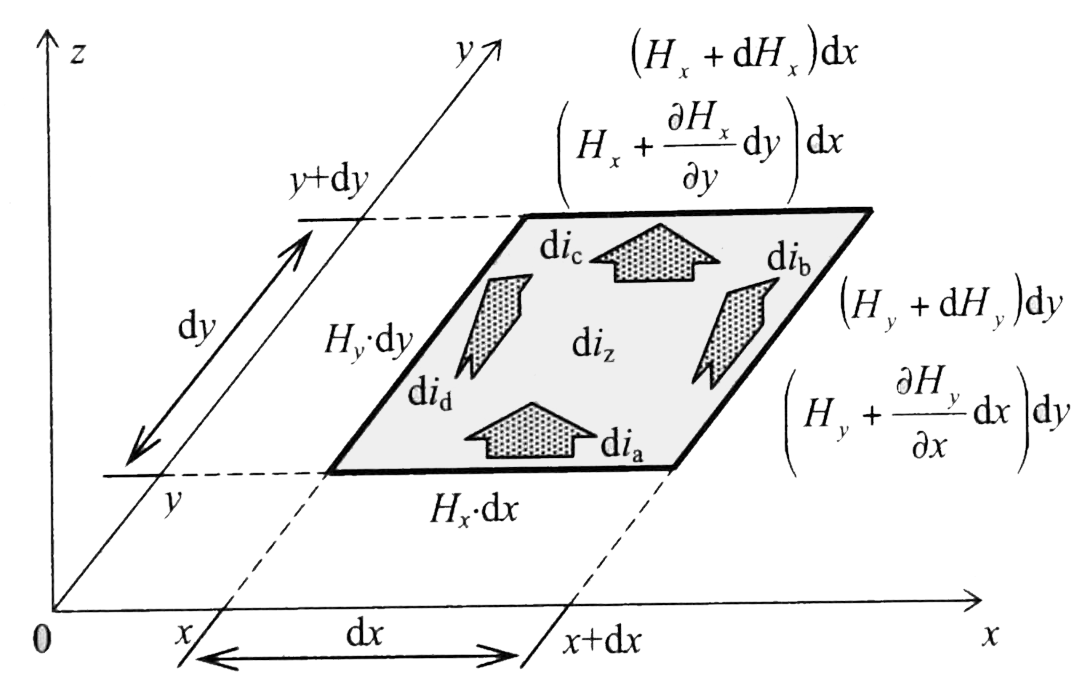
\includegraphics[width=0.8\linewidth]{patocka_mag_tok_exp12.png}
        \caption{Geometrická interpretace \emph{z}-složky \((\rot{H}_z)\) vektoru \(\rot{H}\).}
        \label{es:fig_patocka_mag_tok_exp12}
      \end{figure}
      Geometrický význam \emph{z}-složky \((\rot{H}_z)\) je zřejmý z obr. 
      \ref{es:fig_patocka_mag_tok_exp12}. Jedná se o podobnou situaci, jaká je zobrazena na Obr. 
      \ref{ES:fig_patocka_mag_tok_exp11a}. S ohledem na diferenciální velikost plochy \(dS_z\) je 
      totiž nutno proudy \(di_a, di_b\) ... chápat jako \emph{spojitě rozprostřené} v ploše 
      \(dS_z\), nikoli jako bodové (menší plocha než \(dS_z\) totiž neexistuje). Elementární proud 
      \(di_z = di_a + di_b + di_c + di_d\) tekoucí diferenciální smyčkou \(dS_z\) se nazývá 
      \textbf{ elementární cirkulací} vektoru \(\vec{H}\).

  \section{Třetí Maxwellova rovnice}\label{ES:sec08}
    Konstrukce třetí Maxwellovy rovnice je založena na pojmu \emph{divergence vektoru}, proto je 
    nezbytné nejdříve se s tímto pojmem seznámit.
    
    \subsection{Divergence vektoru D}\label{ES:ssec01}
      Elektrická indukce \(\vec{D}\) je \emph{vektor}, který má význam lokální \emph{plošné 
      hustoty} \(d\Psi_D/dS\) dielektrického toku \(\Psi_D\) neboli plošné hustoty \(dQ/dS\) náboje 
      \(Q\), protože platí identita \(\Psi\equiv Q\).
      
      Naproti tomu divergence \(\diver{D}\) vektoru je \emph{skalár}, který má význam lokální 
      \emph{objemové hustoty} \(\varrho\) náboje. Chceme-li získat objemovou hustotu \(\varrho\) 
      náboje, musíme každou složku \(D_x, D_y , D_z\) indukce \(\vec{D}\) derivovat podle příslušné 
      proměnné \(x, y, z\). Derivace totiž určuje \emph{přírůstek indukce} a ten musí být způsoben 
      \emph{výskytem lokálního náboje} v daném diferenciálním objemu \(dV\). Pro složku \(D_x\) 
      vektoru \(\vec{D}\) zřejmě podle obr. \ref{es:fig_patocka_mag_tok_exp13} platí:
      \begin{equation}\label{ES:eq_zakl_elm46}
        D_x = \frac{d\Psi_{D_x}}{dS_x} = \frac{d\Psi_{D_x}}{\dd{y}\,\dd{z}} = \frac{dQ_x}{\dd{y}\,\dd{z}}. 
      \end{equation} 
      Divergenci ve směru \(x\) získáme tak, že složku indukce \(D_x\) derivujeme podle příslušné 
      proměnné \(x\). S pomocí rovnice (\ref{ES:eq_zakl_elm46}) lze derivaci \(\frac{dD_x}{\dd{x}}\) 
      vyjádřit ve tvaru
      \begin{equation}\label{ES:eq_zakl_elm47}
        (\diver{D})_x = \frac{dD_x}{dS_x} = \frac{dQ_x}{\dd{x}\dd{y}\dd{z}} = \frac{dQ_x}{dV} = \varrho_x. 
      \end{equation} 
      Podobně můžeme získat složky divergence ve zbývajících směrech. Z rovnice 
      (\ref{ES:eq_zakl_elm47}) vyplývá, jak souvisí přírůstek indukce \(dD_x\) s objemovou hustotou 
      \(\varrho_x\) náboje a s divergenci. Na výstupu elementární krychle bude mít přírůstek 
      indukce ve směru \(x\) velikost
      \begin{equation}\label{ES:eq_zakl_elm48}
        dD_x = \varrho_x\,\dd{x} = (\diver{D})_x\,\dd{x} = \pder{D_x}{x}\,\dd{x}. 
      \end{equation} 
      \begin{figure}[ht!]
        \centering
        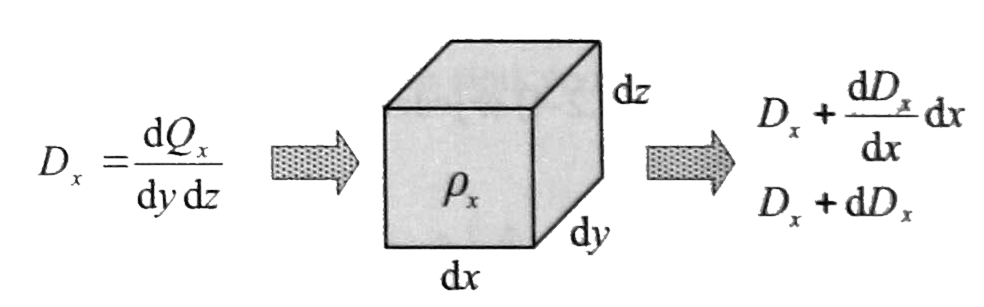
\includegraphics[width=0.9\linewidth]{patocka_mag_tok_exp13.png}
        \caption{Vztah mezi složkou elektrické indukce \(D_x\) a objemovou hustotou \(\varrho_x\) 
                 náboje.}
        \label{es:fig_patocka_mag_tok_exp13}
      \end{figure}
      
      Hustota náboje je \emph{skalární aditivní} veličina. Proto musíme algebraicky sečíst 
      příspěvky \(\varrho_x, \varrho_y, \varrho_z\) ode všech složek divergence ve směrech \(x, y, 
      z\), abychom získali celkovou hustotu \(\varrho\) náboje v elementárním objemu. Celkové 
      hustotě bude rovna i celková divergence v daném bodě:
      \begin{align}\label{ES:eq_zakl_elm49}
        \diver{D} &= (\diver{D})_x + (\diver{D})_y + (\diver{D})_z  \nonumber \\
                  &= \pder{D_x}{x} + \pder{D_y}{y} + \pder{D_z}{z} =
                     \varrho_x + \varrho_y + \varrho_z = \varrho. 
      \end{align} 
      Objemová hustota náboje, tedy i divergence, jsou \emph{skalární} veličiny.
      
    \subsection{Konstrukce třetí Maxwellovy rovnice}\label{ES:ssec02}
      Rovnice (\ref{ES:eq_zakl_elm49}) je přímo III. Maxwellovou rovnicí v diferenciálním tvaru:
      \begin{equation}\label{ES:eq_zakl_elm50}
        \diver{D} = \varrho \qquad [C/m^2, 1/m; C/m^3]. 
      \end{equation} 
      \begin{figure}[ht!]
        \centering
        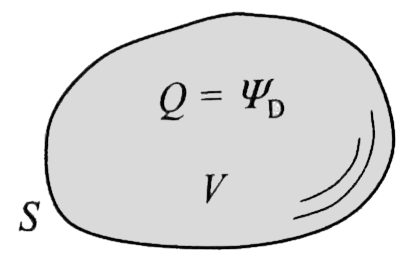
\includegraphics[width=0.4\linewidth]{patocka_mag_tok_exp14.png}
        \caption{Uzavřená orientovaná plocha \(S\) (např. koule) tvoří hranici vnitřního prostoru o 
                 objemu \(V\). Ve vnitřním prostoru se nachází náboj \(Q\).}
        \label{es:fig_patocka_mag_tok_exp14}
      \end{figure}
      
      Plocha \(S\) na obr \ref{es:fig_patocka_mag_tok_exp14} tvoří hranici vnitřního prostoru o 
      objemu \(V\). Z topologického hlediska se jedná o plochu \emph{neohraničenou} (nemá hraniční 
      křivku \(l\)) a \emph{orientovanou} (vnitřní stěnu lze natřít zeleně \textbf{z}, vnější 
      červeně \textbf{č}). Příkladem plochy může být \emph{koule}. Celkový dielektrický tok 
      \(\Psi_D\) prostupující plochou je roven celkovému náboji \(Q\) uvnitř plochy. Pro tok 
      \(\Psi_D\) platí analogie rovnic (\ref{ES:eq_zakl_elm12}), (\ref{ES:eq_zakl_elm39}), a to 
      včetně věty \ref{es:fig_patocka_lemma01} o nezávislosti integrálu na tvaru plochy:
      \begin{equation}\label{ES:eq_zakl_elm51}
        \Psi_D \equiv Q = \int_S\vec{D}\cdot \dd{\vec{S}}.
      \end{equation} 
      Plošný integrál (\ref{ES:eq_zakl_elm51}) převedeme pomocí \textbf{Gaussovy 
      věty}\footnote{Gaussovu větu vysvětlíme v následující kapitole} na integrál objemový:
      \begin{equation}\label{ES:eq_zakl_elm52}
        \Psi_D \equiv Q = \int_S\vec{D}\cdot \dd{\vec{S}} = \int_V\diver{D}\,dV.
      \end{equation} 
      Do rovnice (\ref{ES:eq_zakl_elm52}) dosadíme místo divergence \(\diver{D}\) pravou stranu 
      rovnice (\ref{ES:eq_zakl_elm50}), tj. nábojovou hustotu \(\varrho\). Tak získáme \emph{III. 
      Maxwellovu rovnici} v \emph{integrálním} tvaru
      \begin{equation}\label{ES:eq_zakl_elm53}
        \boxed{\int_S\vec{D}\cdot \dd{\vec{S}} = \int_V\varrho\,dV}.
      \end{equation} 
      Zdůrazněme, že na levé straně rovnice (\ref{ES:eq_zakl_elm53}) se jedná o skalární součin 
      dvou vektorů, na pravé straně o prostý součin dvou skalárů.
      
    \subsection{Gaussova věta}
      Plocha \(S\) tvoří podle obr. \ref{es:fig_patocka_mag_tok_exp14} hranici vnitřního prostoru o 
      objemu \(V\). Z topologického hlediska se jedná o plochu \emph{neohraničenou} a 
      \emph{orientovanou} (např. koule). Gaussova\footnote{Carl Fridrich Gauss (1777-1855), 
      vynikající matematik a fyzik, působil na univerzitě v Gottingenu. Kromě matematiky a 
      elektřiny se zabýval např. teorií geomagnetismu. Společně s W. E. Weberem sestrojili r. 1833 
      první telegraf.}  věta obecně převádí plošný integrál přes tuto plochu \(S\) na objemový 
      integrál přes objem \(V\). Pro pochopení věty velice pomáhá konkrétní fyzikální interpretace 
      jednotlivých veličin. Proto budeme větu zkoumat v konkrétním případě pro vektor indukce 
      \(\vec{D}\). Pak má věta tvar
      \begin{equation}\label{ES:eq_zakl_elm54}
        \int_S\vec{D}\cdot \dd{\vec{S}} = \int_V\diver{D}\,dV \quad(=Q).
      \end{equation} 
      Jak plyne z rovnic (\ref{ES:eq_zakl_elm51}), (\ref{ES:eq_zakl_elm52}), obě strany rovnice 
      (\ref{ES:eq_zakl_elm54}) mají význam celkového náboje \(Q\) uzavřeného uvnitř plochy. Důkaz 
      věty lze konstruovat tak, že \emph{trojný objemový} integrál na pravé straně rovnice 
      (\ref{ES:eq_zakl_elm54}) se budeme snažit převést nezávislým matematickým postupem na dvojný 
      plošný integrál. Z rovnice (\ref{ES:eq_zakl_elm49}) plyne
      \begin{equation}\label{ES:eq_zakl_elm55}
        \varrho = \varrho_x + \varrho_y + \varrho_z 
                = \der{D_x}{x} + \der{D_y}{y} + \der{D_z}{z}. 
      \end{equation}
      Pravou stranu rovnice (\ref{ES:eq_zakl_elm54}) vyjádříme ve tvaru trojného integrálu a 
      dosadíme do ní místo \(\varrho\) pravou stranu rovnice (\ref{ES:eq_zakl_elm55}):
      \begin{align}\label{ES:eq_zakl_elm56}
        Q &= \int_V\diver{D}dV = \int_V\varrho dV 
           = \limitint_{\mathclap{x_Vy_Vz_V}}\varrho\,\dd{x}\,\dd{y}\,\dd{z}   \nonumber\\
          &= \limitint_{\mathclap{x_Vy_Vz_V}}\left(dD_x\,\dd{y}\,\dd{z}+dD_y\,\dd{x}\,\dd{z}+dD_z\,\dd{x}\,\dd{y}\right).
      \end{align}      
      \begin{figure}[ht!]
        \centering
        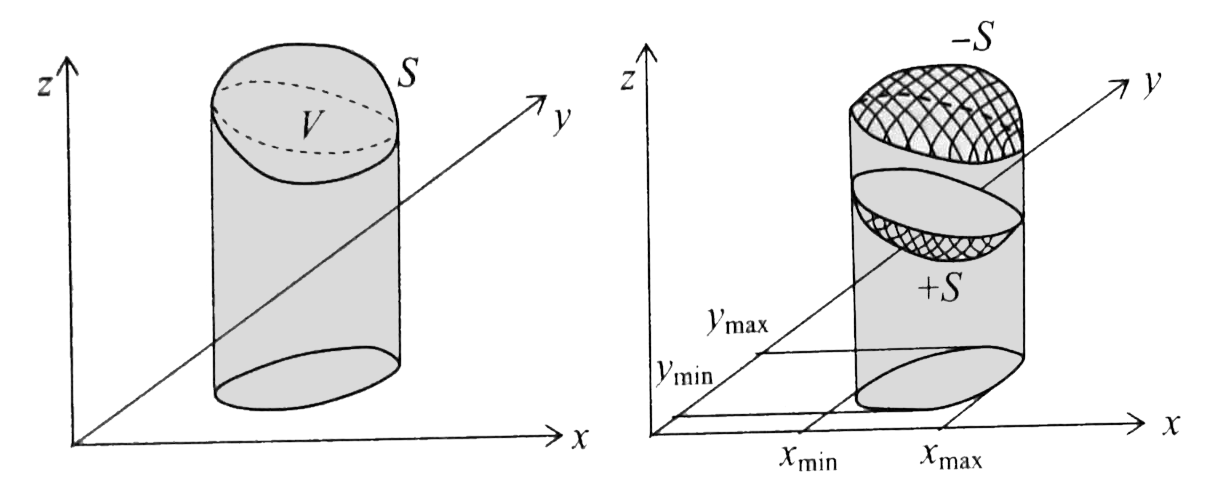
\includegraphics[width=0.9\linewidth]{patocka_mag_tok_exp15.png}
        \caption{Průmět uzavřené plochy \(S\) do roviny \emph{x-y}. Průměty do roviny \emph{y-z, 
                 z-x} lze získat podobně.}
        \label{es:fig_patocka_mag_tok_exp15}
      \end{figure}
      Integrační meze \(x_Vy_Vz_V\) odpovídají podle obr. \ref{es:fig_patocka_mag_tok_exp15} 
      průmětům prostoru \(V\) do příslušných souřadných rovin a z nich do příslušných souřadných 
      os. Zřejmě platí
      \begin{equation}\label{ES:eq_zakl_elm57}
        \limitint_{\mathclap{x_V}}dD_x = D_x \qquad
        \limitint_{\mathclap{y_V}}dD_y = D_y \qquad
        \limitint_{\mathclap{z_V}}dD_z = D_z.
      \end{equation}
      Po dosazení rovnic (\ref{ES:eq_zakl_elm57}) do (\ref{ES:eq_zakl_elm56}) získáme výraz
      \begin{align}\label{ES:eq_zakl_elm58}
        Q &= \iiint\limits_{x_Vy_Vz_V}\varrho\,\dd{x}\,\dd{y}\,\dd{z}   \nonumber\\ 
          &= \iint\limits_{y_Vz_V}D_x\,\dd{y}\,\dd{z} + 
             \iint\limits_{z_Vx_V}D_y\,\dd{z}\,\dd{x} + 
             \iint\limits_{x_Vy_V}D_z\,\dd{x}\,\dd{y}               \nonumber\\ 
          &= \int\limits_{S_x}D_x\,dS_x + 
             \int\limits_{S_y}D_y\,dS_y + 
             \int\limits_{S_z}D_z\,dS_z =  \int\limits_{S}\vec{D}\cdot\vec{S}
      \end{align}
      Ve třech dílčích integrálech nefiguruje součin skalární, nýbrž součin prostý (jedná se o 
      složky vektoru, nikoli o vektor). Integrační meze \(S_x, S_y, S_z\) mají význam 
      \emph{průmětů} plochy \(S\) do jednotlivých souřadných rovin \(y-z\), \(z-x\), \(x-y\). 
      Protože je plocha \(S\) uzavřená, v příslušné rovině existují vždy dva různé průměty: 
      \(S_{+x}, S_{-x}, S_{+y}, S_{-y}, S_{+z}, S_{-z}\). Těm odpovídají dvě různé indukce: 
      \(D_{+x}, D_{-x}, D_{+y}, D_{-y}, D_{+z}, D_{-z}\). V rovnici (\ref{ES:eq_zakl_elm58}) se 
      tedy ve skutečnosti objeví šest dílčích plošných integrálů, uspořádaných do tří dvojic:
      \begin{align*}   %\label{ES:eq_zakl_elm59}
        Q  = \iiint\limits_{x_Vy_Vz_V}\varrho\,\dd{x}\,\dd{y}\,\dd{z}   
          &= \int\limits_{S_x}D_x\,dS_x + 
             \int\limits_{S_y}D_y\,dS_y + 
             \int\limits_{S_z}D_z\,dS_z                                                \\
          &= \int\limits_{S_{+x}}D_{+x}\,dS_x - \int\limits_{S_{-x}}D_{-x}\,dS_x       \\
          &+ \int\limits_{S_{+y}}D_{+y}\,dS_y - \int\limits_{S_{-y}}D_{-y}\,dS_y       \\
          &+ \int\limits_{S_{+z}}D_{+z}\,dS_z - \int\limits_{S_{-z}}D_{-z}\,dS_z       \\
          &= \underbrace{\iint\limits_{y_Vz_V}D_{+x}\,\dd{y}\,\dd{z} 
           - \iint\limits_{y_Vz_V}D_{-x}\,\dd{y}\,\dd{z}}_{\text{dva průměty do roviny y-z}}   \\
          &+ \underbrace{\iint\limits_{z_Vx_V}D_{+y}\,\dd{z}\,\dd{x} 
           - \iint\limits_{z_Vx_V}D_{-y}\,\dd{z}\,\dd{x}}_{\text{dva průměty do roviny z-x}}   \\
          &+ \underbrace{\iint\limits_{x_Vy_V}D_{+z}\,\dd{x}\,\dd{y} 
           - \iint\limits_{x_Vy_V}D_{-z}\,\dd{x}\,\dd{y}}_{\text{dva průměty do roviny x-y}}
      \end{align*}
      Záporná znaménka u sudých integrálů plynou z faktu, že plochy ve dvojici příslušných průmětů 
      jsou opačně orientovány (\textbf{č}\(\rightarrow\)\textbf{z}, 
      \textbf{z}\(\rightarrow\)\textbf{č}). Trojný objemový integrál se tedy podařilo převést 
      na integrál dvojný plošný. Tím je důkaz věty dokončen.
      
  \section{Čtvrtá Maxwellova rovnice}\label{ES:sec09}
    Postup při odvození IV. Maxwellovy rovnice je formálně naprosto shodný s postupem v předchozích 
    kapitolách \ref{ES:ssec01}. a \ref{ES:ssec01}. Ve všech rovnicích pouze nahradíme 
    \emph{elektrické} veličiny analogickými veličinami \emph{magnetickými}, tj. \(D\rightarrow 
    B\), \(\Psi_D\rightarrow \Psi\), \(\varrho\rightarrow \varrho_m\). Proto budou oba 
    tvary IV. MR formálně podobné tvarům III. MR, tj. rovnicím (\ref{ES:eq_zakl_elm53}), 
    (\ref{ES:eq_zakl_elm53}). Velký rozdíl je ale v tom, že elektrické pole je \emph{zřídlové}, 
    kdežto magnetické pole je \emph{vírové}. Z topologického pohledu to znamená:
    \begin{itemize}[noitemsep]
      \item Siločáry elektrické intenzity \(\vec{E}\) nebo \(\vec{D}\) jsou \emph{neuzavřené} 
            křivky, které mají začátek ve „zřídlu“ +Q a konec ve „zřídlu“ -Q.
    
      \item Siločáry magnetické intenzity \(\vec{H}\) nebo \(\vec{B}\) jsou naopak \emph{uzavřené} 
            křivky (tj. „víry“), které  nemají ani začátek ani konec, protože neexistuje magnetický 
            náboj v podobě magnetického monopolu. V magnetismu tedy neexistuje analogie v podobě 
            „+zřídla“ a „-zřídla“. Odtud plyne, že objemová hustota magnetických monopolů 
            \(\varrho_m\) je vždy \emph{nulová}, proto musí být v obou rovnicích položeno 
            \(\varrho_m = 0\).
    \end{itemize}
    \emph{Diferenciální tvar} IV. Maxwellovy rovnice tedy bude:
    \begin{equation}\label{ES:eq_zakl_elm60}
      \diver{B} = 0 \qquad [Wb/m^2,1/m; Wb/m^3].
    \end{equation}
    \emph{Integrální tvar} IV. Maxwellovy rovnice bude:
    \begin{equation}\label{ES:eq_zakl_elm61}
      \int_S\vec{B}\cdot \dd{\vec{S}} = 0.
    \end{equation}    
    V rovnici (\ref{ES:eq_zakl_elm61}) se vždy jedná o \emph{uzavřenou neohraničenou orientovanou} 
    plochu \(S\) (např. kouli, jež má vnitřní stěnu natřenu zeleně \textbf{z}, vnější stěnu červeně 
    \textbf{č}), která tvoří hranici vnitřního prostoru o objemu \(V\), viz obr. 
    \ref{ES:fig_patocka_mag_tok_exp16}. Ve vnitřním prostoru se nemůže nacházet magnetický náboj 
    \(Q_m = \Psi\) v podobě magnetického monopolu - chybí tam zdroj siločar.
   
    \begin{figure}[ht!]
      \centering  
      \subcaptionbox{\label{ES:fig_patocka_mag_tok_exp16a}}{\luafigure[0.45]{patocka_mag_tok_exp16a.png}}
      \subcaptionbox{\label{ES:fig_patocka_mag_tok_exp16b}}{\luafigure[0.45]{patocka_mag_tok_exp16b.png}}
      \caption{Uzavřená orientovaná plocha \(S\) tvořící hranici vnitřního prostoru \(V\): a)   
               ve vnitřním prostoru se nemůže nacházet magnetický náboj \(Q_m = \Phi\) v podobě 
               magnetického monopólu, b) vnější tok vstupuje do vnitřního prostoru levou části 
               plochy ve směru \textbf{č\(\rightarrow\)z} a vystupuje pravou částí ve směru 
               \textbf{z\(\rightarrow\)č}.} 
      \label{ES:fig_patocka_mag_tok_exp16}
    \end{figure}

    Všechny vnější siločáry vstupují do vnitřního objemu částí plochy ve směru 
    \textbf{č}\(\rightarrow\)\textbf{z} a vystupují ven zbývající částí ve směru 
    \textbf{z}\(\rightarrow\)\textbf{č}. Tyto dvě části lze od sebe formálně oddělit uzavřenou 
    křivkou \(l\), která tvoří přirozenou hranici mezi těmito dvěma oblastmi - jedná se o 
    geometrické místo tečných bodů, v nichž se některé ze siločar pouze tečné dotknou plochy \(S\), 
    aniž ji protnou. Pak je možno na problém aplikovat větu \ref{es:fig_patocka_lemma01}: Integrál 
    přes oblast \textbf{č}\(\rightarrow\)\textbf{z} musí mít v absolutní hodnotě stejnou 
    velikost jako integrál přes oblast \textbf{z}\(\rightarrow\)\textbf{č}. S ohledem na opačné 
    orientace však musí mít oba integrály navzájem opačná znaménka. Proto musí platit:
    \begin{equation}\label{ES:eq_zakl_elm62}
      \int\limits_{S}\vec{B}\cdot \dd{\vec{S}} = 
      \int\limits_{\text{č}\rightarrow\text{z}}\vec{B}\cdot \dd{\vec{S}} -
      \int\limits_{\text{z}\rightarrow\text{č}}\vec{B}\cdot \dd{\vec{S}} = 0.
    \end{equation} 
    Celkový tok plochou \(S\) je tedy opravdu nulový.
    
  \section{Biotův-Savartův zákon}\label{ES:sec10}
    Oersted\footnote{Hans Christian Oersted (1777-1851), fyzik a chemik, působil na univerzitě v 
    Kodani. Ve víře v jednotnou přírodní sílu hledal souvislosti mezi přírodními jevy na první 
    pohled nesouvisejícími.} zveřejnil v roce 1820 své experimentální výsledky, týkající se 
    silového působení elektrického proudu na magnetku kompasu. Jeho výsledky však byly pouze 
    kvalitativní. Zanedlouho poté odvodili Biot\footnote{Jean Baptisté Biot (1774-1862), fyzik, 
    působil na Sorboně. Zabýval se elektrodynamikou a optikou.} se Savartem\footnote{Felix Savart 
    (1791-1841), lékař, později působil jako fyzik na Sorboně. Zabýval se elektrodynamikou a 
    akustikou.} na základě složitých experimentů kvantitativní vztah pro výpočet síly působící na 
    magnetku, který upravil Laplace do tvaru
    \begin{equation}\label{ES:eq_zakl_elm63}
      d\vec{F} = KI\frac{\dd{\vec{l}}\times \vec{r}}{r^3}
    \end{equation} 
    
    Konstanta \(K\) v Laplaceově\footnote{Pierre-Simon Laplace (1749-1827), matematik a astronom, 
    člen francouzské Akademie věd. Zabýval se mechanikou a gravitační stabilitou sluneční soustavy, 
    teorií potenciálu, je zakladatelem integrálních transformací v matematice.} rovnici je závislá 
    na použité soustavě jednotek. Zákon říká, že každá elementární část vodiče o diferenciální 
    délce \(dl\) působí na magnetku diferenciálním přírůstkem síly \(dF\). Oersted však zjistil, že 
    vodič \(L\) působí zcela stejně nejen na magnetku, ale i na malý kruhový závit, kterým protéká 
    jiný nezávislý proud. Na základě tohoto experimentálního faktu bylo možno o několik let 
    později, až po zavedení pojmu \emph{„magnetické pole“} Faradayem, modifikovat Biotův-Savartův 
    zákon do současné podoby. Současný tvar zákona, daný rovnicí (\ref{ES:eq_zakl_elm63}), umožňuje 
    výpočet magnetického pole \(H\) nebo \(B\), generovaného vodičem libovolného tvaru, v 
    libovolném bodě prostoru. Prostor ale musí být vyplněn magneticky \emph{izotropním, homogenním 
    a lineárním} prostředím. Předpokladem je, že tloušťka vodiče je zanedbatelná vůči rozměrům 
    vyšetřovaného prostoru. Zákon říká, že každá část vodiče o diferenciální délce \(dl\) vytváří 
    ve sledovaném bodě diferenciální přírůstek magnetického pole \(dH\), resp. \(dB\) podle rovnice
    \begin{equation}\label{ES:eq_zakl_elm64}
      d\vec{H} = \frac{I}{4\pi}\frac{\dd{\vec{l}}\times \vec{r}}{r^3}, \qquad\text{resp.}\qquad
      d\vec{B} = \mu_0\frac{I}{4\pi}\frac{\dd{\vec{l}}\times \vec{r}}{r^3}.
    \end{equation}     
    \begin{figure}[ht!]
      \centering
      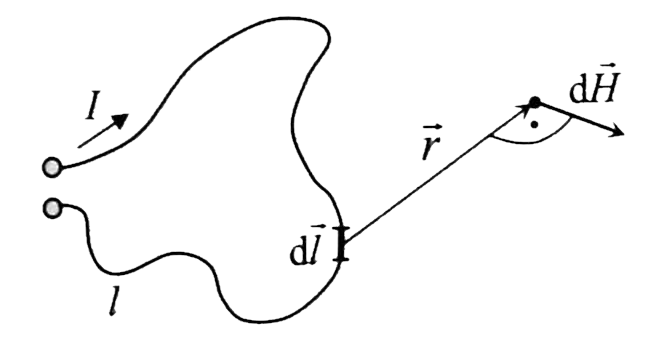
\includegraphics[width=0.5\linewidth]{patocka_mag_tok_exp17.png}
      \caption{K Biotovu-Savartovu zákonu.}
      \label{es:fig_patocka_mag_tok_exp17}
    \end{figure}
    Celkové pole v tomtéž sledovaném bodě lze určit integrací diferenciálních přírůstků 
    (\ref{ES:eq_zakl_elm64}), způsobených všemi diferenciálními částmi \(dl\) vodiče. Konečná 
    podoba Biotova-Savartova zákona má tvar křivkového integrálu, přičemž integrační křivka \(l\) 
    je určena tvarem vodiče:
    \begin{equation}\label{ES:eq_zakl_elm65}
      \vec{H} = \frac{I}{4\pi}\int_l\frac{\dd{\vec{l}}\times \vec{r}}{r^3}, \quad\text{resp.}\quad
      \vec{B} = \mu_0\frac{I}{4\pi}\int_l\frac{\dd{\vec{l}}\times \vec{r}}{r^3}.
    \end{equation} 
    
    Pro obecný tvar vodiče je výpočet křivkového integrálu tak složitý, že je obvykle v uzavřeném 
    tvaru neřešitelný. Snadno řešitelný je však ve \emph{zvláštních případech}, které vykazují 
    vhodnou geometrickou symetrii.
    
    Jedním z nich je výpočet pole \emph{přímého nekonečně dlouhého vodiče}. Je známo, že pole 
    \(\vec{H}\) takového vodiče je kruhově symetrické podle obr. 
    \ref{es:fig_patocka_mag_tok_exp18}. Pro bod umístěný ve vzdálenosti \(R\) od vodiče lze 
    druhou rovnici (\ref{ES:eq_zakl_elm64}) modifikovat do tvaru      
    \begin{figure}[ht!]
      \centering
      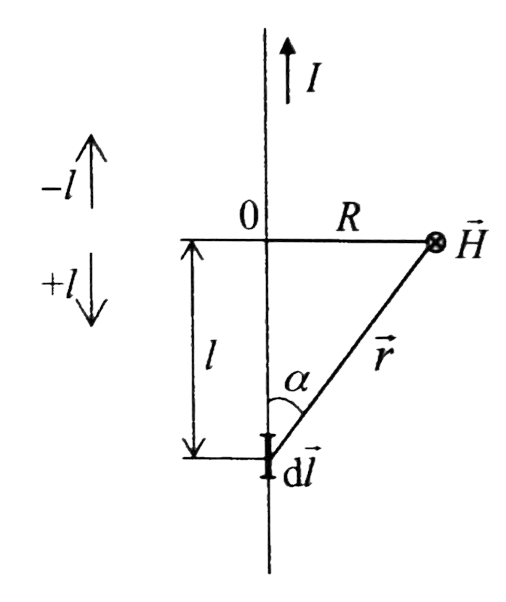
\includegraphics[width=0.4\linewidth]{patocka_mag_tok_exp18.png}
      \caption{K výpočtu pole přímého nekonečně dlouhého vodiče pomocí Biotova-Savartova zákona.}
      \label{es:fig_patocka_mag_tok_exp18}
    \end{figure}
    \begin{align}\label{ES:eq_zakl_elm66}
      d\vec{H} &= \frac{I}{4\pi}\frac{dl\,r\sin\alpha}{r^3}
                = \frac{I}{4\pi}\frac{dl\sin\alpha}{r^2}                 \nonumber \\
               &= \frac{I}{4\pi}\frac{Rdl}{r^3}
                = \frac{IR}{4\pi}\frac{dl}{\left(r^2+l^2\right)^{\frac{3}{2}}}
    \end{align}
    Podle rovnice (\ref{ES:eq_zakl_elm65}) pro \(\vec{H}\) bude mít intenzita magnetického pole 
    velikost 
    \begin{align}\label{ES:eq_zakl_elm67}
      \vec{H} &= \frac{IR}{4\pi}\int\limits_{-\infty}\limits^{+\infty}
                 \frac{dl}{\left(r^2+l^2\right)^{\frac{3}{2}}}
               = \frac{IR}{4\pi} 
                 \left[\frac{l}{R^2\sqrt{R^2+l^2}}\right]_{-\infty}^{+\infty}         \nonumber \\
              &= \frac{I}{4\pi R}
                 \left[\frac{1}{\sqrt{\dfrac{R^2}{l^2}+1}}\right]_{-\infty}^{+\infty} \nonumber \\
              &= \frac{I}{4\pi R}[1-(-1)] = \frac{I}{2\pi R}
    \end{align}
    Poznamenejme, že po krácení zlomku v prvních hranatých závorkách veličinou \(l\) nesmí 
    zaniknout informace o znaménku veličiny \(l\). Proto musí být hodnota následného zkráceného 
    zlomku ve druhých hranatých závorkách po dosazení dolní meze \emph{záporná}, po dosazení horní 
    meze \emph{kladná}. Takto jsme dospěli ke známému výsledku pro intenzitu magnetického pole 
    přímého dlouhého vodiče. Této intenzitě odpovídá magnetická indukce
    \begin{equation}\label{ES:eq_zakl_elm68}
      B = \mu_0H = \mu_0\frac{I}{2\pi R}
    \end{equation}
    
    Jiným zvláštním případem, vykazujícím geometrickou symetrii, je výpočet pole v rotační ose 
    kruhového závitu nebo válcové cívky ( např. \emph{Helmholtzovy cívky}). 
    
  \section{Elektromagnetické síly}\label{ES:sec11}
    Cílem této kapitoly je ukázat jednotné fyzikální principy vedoucí ke vzniku mechanických sil.
    
    \subsection{Vznik mechanických sil v elektromagnetickém poli}
      Koná-li síla \(F\) práci na dráze \(l\) a mění-li během pohybu svoji velikost, nelze použít k 
      výpočtu mechanické práce rovnici \(W_{mech}= Fl\), nýbrž je nutno použít její diferenciální 
      obdobu
      \begin{equation}\label{ES:eq_zakl_elm69}
        dW_{mech} = Fdl
      \end{equation}
      
      Platnost rovnice je založena na základním principu diferenciálního počtu, který říká, že v 
      limitním případě, na diferenciální dráze \(dl\), musí být síla \(F\) \emph{konstantní}. S 
      ohledem na \emph{limitně nulovou} délku dráhy \(dl\) se diferenciální přírůstek vykonané 
      práce \(dW_{mech}\) též někdy nazývá \textbf{virtuální prací}. Virtuální práce \(dW_{mech}\), 
      vykonaná izolovanou fyzikální soustavou, musí být kryta ze zdroje energie energetickým 
      příspěvkem \(dW\), a to takovým způsobem, aby \emph{celková energie soustavy zůstala 
      zachována}. Odtud plyne, že součet diferenciálních energetických přírůstků v izolované 
      soustavě musí být nulový:
      \begin{equation}\label{ES:eq_zakl_elm70}
        dW_{mech}+dW=0.
      \end{equation}
      Z rovnic (\ref{ES:eq_zakl_elm69}), (\ref{ES:eq_zakl_elm70}) plyne, že v soustavě nutně vzniká 
      mechanická síla
      \begin{equation}\label{ES:eq_zakl_elm71}
        \boxed{F = \frac{dW_{mech}}{dl} = -\frac{dW}{dl}},
      \end{equation}
      kde \(dW\) je přírůstek energie dodaný zdrojem.
      
      V případě elektromagnetu se železným jádrem a se vzduchovou mezerou lze zanedbat magnetickou 
      vodivost železa oproti vodivosti vzduchové mezery. Pak je veškerá magnetická energie 
      soustředěna pouze do objemu vzduchové mezery o délce \(l\):
      \begin{equation}\label{ES:eq_zakl_elm72}
        W =\frac{1}{2}Li^2 = \frac{1}{2}i^2N^2\mu_0\frac{S_{Fe}}{l}.
      \end{equation}
      Z rovnic (\ref{ES:eq_zakl_elm72}) a (\ref{ES:eq_zakl_elm71}) plyne, že ve vzduchové mezeře 
      magnetu vznikne síla
      \begin{align}\label{ES:eq_zakl_elm73}
         F = -\frac{dW}{dl} 
           &= +\frac{1}{2}i^2N^2\mu_0\frac{S_{Fe}}{l^2}
           =  \frac{1}{2}i^2\frac{L}{l} = \frac{1}{2}H^2\mu_0S_{Fe}              \nonumber \\
           &=  \frac{1}{2}BHS_{Fe} = \frac{1}{2}\frac{B^2}{\mu_0}S_{Fe}.
      \end{align}
      Mechanický tlak ve vzduchové mezeře bude
      \begin{equation}\label{ES:eq_zakl_elm74}
        p = \frac{F}{S_{Fe}} = \frac{1}{2}H^2\mu_0 = \frac{1}{2}BH = \frac{1}{2}\frac{B^2}{\mu_0}.
      \end{equation}
      Z rovnice (\ref{ES:eq_zakl_elm72}) rovněž vyplývá, že objemová hustota energie magnetického 
      pole ve vzduchové mezeře je \emph{identicky rovna} mechanickému tlaku:
      \begin{align}\label{ES:eq_zakl_elm75}
        w  = \frac{W}{V} 
          &= \frac{W}{S_{Fe}l} = \frac{1}{2}i^2N^2\mu_0\frac{1}{l^2}             \nonumber \\
          &= \frac{1}{2}H^2\mu_0 = \frac{1}{2}BH = \frac{1}{2}\frac{B^2}{\mu_0}.
      \end{align}
      Podobně v případě vzduchového kondenzátoru lze sílu určit pomocí elektrostatické energie 
      nashromážděné v prostoru mezi elektrodami:
      \begin{equation}\label{ES:eq_zakl_elm76}
        W = \frac{1}{2}u^2C = \frac{1}{2}u^2\varepsilon_0\frac{S}{l}.
      \end{equation}
      Z rovnic (\ref{ES:eq_zakl_elm76}) a (\ref{ES:eq_zakl_elm71}) plyne, že ve vzduchové mezeře 
      kondenzátoru vznikne síla
      \begin{align}\label{ES:eq_zakl_elm77}
        F  = \frac{dW}{dl} 
          &= \frac{1}{2}u^2\varepsilon_0\frac{S}{l^2}
           = \frac{1}{2}E^2\varepsilon_0S                                 \nonumber \\
          &= \frac{1}{2}DES           
           = \frac{1}{2}\frac{D^2}{\varepsilon_0}S.
      \end{align}
      Mechanický tlak mezi elektrodami kondenzátoru bude
      \begin{align}\label{ES:eq_zakl_elm78}
        F  = \frac{dW}{dl} 
          &= \frac{1}{2}u^2\varepsilon_0\frac{S}{l^2}
           = \frac{1}{2}E^2\varepsilon_0S                                 \nonumber \\
          &= \frac{1}{2}DES          
           = \frac{1}{2}\frac{D^2}{\varepsilon_0}S.
      \end{align}
      Z rovnice (\ref{ES:eq_zakl_elm76}) vyplývá, že objemová hustota energie elektrického pole 
      mezi elektrodami kondenzátoru je identicky rovna mechanickému tlaku:
      \begin{align}\label{ES:eq_zakl_elm79}
        w  = \frac{W}{V} 
          &= \frac{W}{Sl} 
           = \frac{1}{2}u^2\varepsilon_0\frac{1}{l^2}         \nonumber \\
          &= \frac{1}{2}E^2\varepsilon_0 = \frac{1}{2}DE 
           = \frac{1}{2}\frac{D^2}{\varepsilon_0}.
      \end{align}
      Je zajímavé, že v případě elektromagnetu i kondenzátoru je tlak ve vzduchové mezeře roven 
      objemové hustotě energie v téže mezeře, tj. \(p = w\).
      
      Pro dokreslení fyzikálních souvislostí porovnejme tento výsledek s termodynamikou plynů. U 
      plynu uzavřeného v nádobě se celková hustota kinetické energie molekul musí podle
      \emph{ekvipartičního teorému} rovnoměrně rozdělit mezi tři souřadné směry \(x, y, z\), proto 
      by tlak plynu na stěny nádoby měl být třetinový, ve skutečnosti je ze složitějších důvodů 
      dvoutřetinový oproti hustotě kinetické energie:
      \begin{equation}\label{ES:eq_zakl_elm80}
        p = \frac{2}{3}w
      \end{equation}
      V mezeře elektromagnetu i kondenzátoru vzniká tlak pouze v \emph{jediném} 
      směru\footnote{Předpokládáme, že pólové nástavce jsou v zákrytu. Při vychýleni jednoho z 
      nástavců do strany sice vznikne v mezeře i boční síla, ale to je zcela jiné geometrické 
      uspořádání, které neuvažujeme.}, proto platí \(p = w\). Nositelé \emph{elektromagnetických 
      silových interakcí} jsou fotony\footnote{Na této skutečnosti je založena Feynmanova teorie 
      kvantové elektrodynamiky.}. Ty plní ve vzduchové mezeře elektromagnetu nebo 
      kondenzátoru podobnou roli jako molekuly plynu v nádobě. Rozdíl je pouze v tom, že vznikající 
      síla je přitažlivá, nikoli odpudivá a že fotony působí v jediném směru (při dané geometrické 
      konfiguraci).
      
      Analogicky k rovnici (\ref{ES:eq_zakl_elm74}) lze určit mechanický tlak uvnitř železného 
      jádra elektromagnetu, lokalizovaný ve \emph{vnitřním objemu železa} o relativní permeabilitě 
      \(\mu_{r_{Fe}}\)
      \begin{equation}\label{ES:eq_zakl_elm81}
       p = \frac{1}{2}\frac{B^2}{\mu_0\mu_{r_{Fe}}}.
      \end{equation}
      Vnitřní mechanický tlak v železe je vnějšímu pozorovateli experimentálně nedostupný. Nicméně 
      existuje a vidíme, že je řádově 2000krát menší oproti tlaku v mezeře. Stejný je i poměr 
      hustot energií v železe a v mezeře. To nás plně oprávnilo k původnímu zanedbání železa při 
      výpočtu síly. Všimněme si, že při \emph{konstantním} toku \(\Phi = BS_{Fe} = \text{konst}\). 
      platí tyto zákonitosti:
      \begin{itemize}[noitemsep]
        \item Magnetická síla je tím menší, čím je permeabilita obvodu větší, viz rovnice     
              (\ref{ES:eq_zakl_elm81}).
        \item Magnetická síla je tím menši, čím je plocha \(S_{Fe}\) obvodu větší, viz rovnice 
              (\ref{ES:eq_zakl_elm73}). Zřejmě totiž platí \(F \cong B^2S_{Fe} = 
              \frac{\Phi^2}{S_{Fe}} = \frac{\text{konst.}}{S_{Fe}}\).
      \end{itemize}
      Obě zákonitosti lze zobecnit takto:
      \begin{itemize}[noitemsep]
        \item Magnetická síla, tedy i potenciální energie soustavy, je tím menší, čím větší je    
              magnetická vodivost obvodu.
        \item Tlakové pole vznikající v magnetickém obvodu zaujme vždy takové prostorové rozložení, 
              které se snaží zdeformovat obvod do tvaru, v němž je potenciální energie obvodu co 
              nejmenší\footnote{Z podobných důvodů působí síla na těleso umístěné v gravitačním 
              poli. Gravitační síla má takový směr. že se snaží zmenšit potenciální energii \(mgh\) 
              tělesa na nulu.}, tj. v němž je magnetická vodivost obvodu co největší.
      \end{itemize}
      
      V důsledku obou zobecněných zákonitostí vznikají následující jevy:
      \begin{itemize}[noitemsep]
        \item Je-li součástí obvodu vzduchová mezera, tlakové pole se snaží zkrátit její délku na 
              nulu.
        \item Proudovodič ve tvaru uzavřené smyčky, umístěný volně v prostoru, se tlakové pole   
              snaží \emph{roztáhnout} do co největší plochy, tj. napnout vodič do kružnice.
        \item Dva paralelní vodiče, kterými protékají proudy \emph{opačných} směrů, se 
              \emph{odpuzuji} (v podstatě se jedná o podlouhlou uzavřenou smyčku z předchozího 
              bodu). U transformátoru se odpuzuje sekundární vinutí od primárního (opačné směry 
              proudů). Podobně vzduchová cívka napájená střídavým proudem se odpuzuje od kovové 
              nemagnetické desky, ve které vznikají vířivé proudy.
        \item Dva paralelní vodiče, kterými protékají proudy \emph{souhlasných} směrů, se 
              \emph{přitahuji}. U transformátoru se vzájemně přitahují závity téhož vinutí.
      \end{itemize}
      
      Z uvedených skutečností je zřejmé, že existence magnetické síly nesouvisí s přítomností 
      železa. V magnetickém obvodu, obsahujícím společně železo i vzduchovou mezeru, plní železo 
      roli pouhého „soustřeďovače siločar“ do objemu vzduchové mezery. V mezeře se pak jedná o 
      silovou interakci čistě mezi magnetickým \emph{polem} a \emph{vakuem}. Pro lepší pochopení 
      elektromagnetických sil je vhodné nahlížet na vakuum jako na „pružný materiál“\footnote{Při 
      řešení teoretických fyzikálních problémů je často užitečný „inženýrský přistup“. Z 
      psychologických důvodů proto není na škodu považovat vakuum za plnohodnotný „konstrukční“ 
      materiál, u kterého známe s jistotou tři jeho materiálové konstanty: \(\varepsilon_0\), 
      \(\mu_0\) a měrnou hmotnost \(\varrho = 0\).}, který je magnetickým polem 
      deformován do takového tvaru, aby magnetická vodivost tohoto „materiálu“ byla co 
      \emph{největší}. Jinak řečeno, aktivní objem vakua je silou nucen zaujmout takový tvar, aby 
      celková potenciální energie pole byla co \emph{nejmenší}.
      
      V	případě \emph{rotačního} pohybuje možno modifikovat rovnici (\ref{ES:eq_zakl_elm71}) pro 
      výpočet \emph{momentu síly}. Stačí vynásobit obě strany rovnice délkou ramena \(r\), na němž 
      síla působí:
      \begin{equation*}
        Fr = \frac{dW_{mech}}{dl}r 
           = \frac{dW_{mech}}{\dfrac{dl}{r}} 
           = \frac{dW_{mech}}{d\alpha}
             \qquad \Longrightarrow
      \end{equation*}
      \begin{equation}\label{ES:eq_zakl_elm82}
        \boxed{M = \frac{dW_{mech}}{d\alpha} = \frac{dW}{d\alpha}}
      \end{equation}
      kde \(\alpha\) je úhel natočení. Rovnice je vhodná pro přímý výpočet momentu všech 
      \emph{reluktančních motorů}, jejichž princip je založen na tom, že magnetická vodivost 
      vzduchové mezery se výrazně mění s úhlem natočení hřídele.
      
      Rovnici (\ref{ES:eq_zakl_elm71}) lze interpretovat tak, že síla je rovna \emph{strmosti}, s 
      jakou se mění energie soustavy v závislosti na změně délkové souřadnice \(l\). Ve složitějším 
      geometrickém uspořádání soustavy lze rovnici (\ref{ES:eq_zakl_elm71}) zobecnit do vektorového 
      tvaru
      \begin{equation}\label{ES:eq_zakl_elm83}
       \vec{F} = -\vec{i}\frac{dW}{\dd{x}} -\vec{j}\frac{dW}{\dd{y}} -\vec{k}\frac{dW}{\dd{z}} 
               = - \grad{W},
      \end{equation}
      kde \(\vec{i}, \vec{j}, \vec{k},\) jsou jednotkové vektory ve směru příslušných os. Síla je 
      pak nejobecněji definována jako záporně vzatý gradient (vektor) ze skalární funkce 
      \(W(x,y,z)\).
      
    \subsection{Lorentzova síla}
      
      Elektromagnetické síly působící na elektrický náboj lze shrnout do jediné Lorentzovy rovnice
      \begin{equation}\label{ES:eq_zakl_elm84}
        \vec{F}=q(\vec{E}+\vec{v}\times\vec{B}),
      \end{equation}
      ve které první člen vyjadřuje Coulombovu\footnote{Charles Augustin de Coulomb (1736-1806), 
      absolvent vojenské školy v Paříži. Zákon síly mezi dvěma bodovými náboji odhalil v období 
      1785 až 1789 v soukromí. Později jmenován členem pařížské Akademie věd.} elektrostatickou 
      sílu, působící na náboj \(Q\) umístěný v elektrickém poli \(\vec{E}\) a druhý člen vyjadřuje 
      Lorentzovu\footnote{Henrik Antoon Lorentz (1853-1928), teoretický fyzik, působil na 
      univerzitě v Leidenu. R. 1902 obdržel Nobelovu cenu za fyziku.} sílu, která působí na 
      náboj, pohybující se relativní rychlostí \(v\) vůči magnetickému poli \(B\). Lorentz 
      formuloval obě složky síly zcela obecně, tj. pro náboj pohybující se i relativistickou 
      rychlostí \(v \rightarrow c\), a to pomocí známých Lorentzových transformací. Pro 
      dokreslení historických souvislostí lze dodat, že Coulombův zákon pro náboje pohybující se 
      nižšími nerelativistickými rychlostmi korigoval už Weber ve druhé polovině 19. stol.
      a elektrické pole E, vytvořené relativisticky se pohybujícím nábojem, odvodil 
      Heaviside\footnote{Oliver Heaviside (1850-1925), technik britské telegrafní společnosti, 
      vynálezce duplexního telegrafu. Později soukromý vědec, samouk.} již r. 1888, tj. 17 let před 
      vznikem speciální teorie relativity. 
      
      V běžné inženýrské praxi lze zcela zanedbat Coulombovy síly oproti silám Lorentzovým. Navíc 
      je průměrná transportní (nikoli okamžitá) rychlost volných elektronů v kovech velmi malá, 
      řádově dosahuje \si{\cm/\s}, tudíž není nutno uvažovat relativistické efekty. Pak 
      můžeme uvažovat pouze druhý člen v rovnici (\ref{ES:eq_zakl_elm84}), pomocí něhož lze snadno 
      odvodit elementární Lorentzovu sílu \(dF\), působící na vodič o diferenciální délce \(dl\), 
      který se nachází v magnetickém poli \(B\).
       
      Protéká-li vodičem proud \(I\), z rovnice plyne:
      \begin{equation}\label{ES:eq_zakl_elm85}
        d\vec{F} =  dQ\,\vec{v}\times\vec{B} 
                 = I\dd{t}\,\vec{v}\times\vec{B} 
                 = I\dd{t}\,\frac{\dd{\vec{l}}}{\dd{t}}\times\vec{B}
                 = I\,\vec{l}\times\vec{B}.
      \end{equation}
      Díky vektorovému součinu je síla \(d\vec{F}\) vždy \emph{kolmá} na oba vektory \(\dd{\vec{l}}\) a 
      \(\vec{B}\) a v absolutní hodnotě má velikost
      \begin{equation}\label{ES:eq_zakl_elm86}
              dF=I\,dl\,B\sin\alpha,
      \end{equation}
      kde \(\alpha\) je úhel sevřený oběma vektory \(\dd{\vec{l}}\) a \(\vec{B}\). Proto musí všechny 
      tři vektory v pořadí \(\dd{\vec{l}}\), \(\vec{B}\), \(d\vec{F}\) tvořit \textbf{pravotočivý 
      systém}. Jedná se o \emph{topologickou vlastnost}\footnote{Jednou z několika rozlišitelných 
      topologických kvalit je rozlišení pravé a levé strany.} elektromagnetického pole, která je 
      známa jako \emph{pravidlo levé ruky}.
      \begin{itemize}
        \item \textbf{Pravidlo levé ruky}: Čtyři natažené prsty levé ruky ukazují směr proudu (tj. 
              směr rychlosti náboje), siločáry magnetického pole vstupují do dlaně a palec ukazuje 
              směr síly.
      \end{itemize}

      Předpokládejme, že celý dlouhý vodič je mechanicky dokonale tuhý, nedeformovatelný. Pak 
      celková síla, působící na vodič libovolného tvaru o délce \(l\), bude určena křivkovým 
      integrálem
      \begin{equation}\label{ES:eq_zakl_elm87}
        \vec{F} = \int_ld\vec{F} 
                = I\int_l (\dd{\vec{l}}\times\vec{B}).
      \end{equation}
      Ve \emph{zvláštním} případě, pro přímý vodič o délce \(l\) vložený do \emph{homogenního} 
      magnetického pole \(B\) a orientovaný tak, že vodič je umístěn \emph{kolmo} na směr siločar, 
      dostáváme známý vztah
      \begin{align}\label{ES:eq_zakl_elm88}
        F  =  I\int_l (\dd{\vec{l}}\times\vec{B})
          &= BI\int_l \dd{\vec{l}} = BI\int\limits_{l_1}^{l_2}\dd{\vec{l}}  \nonumber \\
          &= BI[l]_{l_1}^{l_2}
           = BI[l_2 - l_1]
           = BIl.
      \end{align}
      Rovnice (\ref{ES:eq_zakl_elm88}) nachází uplatnění především v teorii stejnosměrných a 
      střídavých strojů. Rovnici lze psát obecněji pro časově proměnné veličiny a navíc modifikovat 
      pro moment síly:
      \begin{equation}\label{ES:eq_zakl_elm89}
        F(t)=B(t)i(t)l, \qquad\text{resp.} \qquad M(t)=B(t)i(t)lr,
      \end{equation}
      kde \(r\) je poloměr vzduchové mezery. V případě stejnosměrného stroje s konstantním buzením, 
      tj. \(B(t) = \text{konst.}\), plyne z rovnice přímá úměra mezi okamžitými hodnotami 
      \emph{proudu} a \emph{momentu} stroje.


    \subsection{Síla mezi dvěma dlouhými rovnoběžnými vodiči}      
      V kapitole \ref{ES:sec10} bylo pomocí Biotova-Savartova zákona odvozeno magnetické pole \(B\) 
      dlouhého přímého vodiče. Siločáry pole máji tvar soustředných kružnic, v jejichž středu leží 
      příslušný vodič. Protéká-li vodičem označeným 1 proud \(I_1\) pak vodič vybudí ve vzdálenosti 
      \(R\) magnetickou indukci
      pro moment síly:
      \begin{equation}\label{ES:eq_zakl_elm90}
        B_1 = \mu_0\frac{I_1}{2\pi R}.
      \end{equation}
      Ve vzdálenosti \(R\) umístíme rovnoběžně s vodičem 1 další vodič, označený 2. Pak se vodič 2 
      nachází v magnetickém poli o velikosti \(B_1\). Protéká-li vodičem 2 proud \(I_2\), pak podle 
      rovnice (\ref{ES:eq_zakl_elm88}) na něj působí síla
       pro moment síly:
      \begin{equation}\label{ES:eq_zakl_elm91}
        F_{1,2} = B_1 I_2 l = \mu_0\frac{I_1}{2\pi R}I_2 l.
      \end{equation}
      Pak měrná síla působící na jednotkovou délku vodiče bude mít velikost
      \begin{equation}\label{ES:eq_zakl_elm92}
        \frac{F_{1,2}}{l} = \mu_0\frac{I_1I_2}{2\pi R}.
      \end{equation}
      Záměnou obou vodičů, tj. záměnou indexů v rovnicích (\ref{ES:eq_zakl_elm90}) a 
      (\ref{ES:eq_zakl_elm91}) lze snadno dokázat, že mezi vodiči platí \emph{zákon akce a reakce} 
      ve tvaru \(F_{1,2} = F_{2,1}\) . Síla je přitažlivá, mají-li oba proudy stejný směr, 
      odpudivá, mají-li směr opačný. Rovnice (\ref{ES:eq_zakl_elm92}) slouží k \emph{dynamické 
      definici} jednotky elektrického proudu \SI{1}{\A}:
      
      Vakuum má z historických důvodů magnetickou permeabilitu
      \begin{equation}\label{ES:eq_zakl_elm93}
        \mu_0= 4\pi\times10^{-7}\,\si{\henry/\m} \cong l,256\times10^{-6}\,\si{\henry/\m}.
      \end{equation}
      Protéká-li oběma rovnoběžnými dlouhými vodiči stejný proud \(I\), síla na jednotku délky 
      vodiče bude mít velikost
      \begin{equation}\label{ES:eq_zakl_elm94}
        \frac{F_{1,2}}{l} = \mu_0\frac{I^2}{2\pi R} = 2\times10^{-7}\frac{I^2}{R}.
      \end{equation}
      Ze změřené síly a vzdálenosti vodičů \(R\) je pak možno určit velikost protékajícího proudu 
      \(I\).
    
%} % tikzset
%~~~~~~~~~~~~~~~~~~~~~~~~~~~~~~~~~~~~~~~~~~~~~~~~~~~~~~~~~~~~~~~~~~~~~~~~~~~~~~~~~~~~~~~~~~~~~~~~~~